\documentclass[review]{elsarticle}

\usepackage{lineno,hyperref}
\modulolinenumbers[5]

\journal{Journal of Computational Physics}

%%%%%%%%%%%%%%%%%%%%%%%
%% Elsevier bibliography styles
%%%%%%%%%%%%%%%%%%%%%%%
%% To change the style, put a % in front of the second line of the current style and
%% remove the % from the second line of the style you would like to use.
%%%%%%%%%%%%%%%%%%%%%%%
%% Math Packages %%%%%%%%%%%%%%%%%%%%%%%%%%%%%%%%%%%%%%%%%%%%
\usepackage{amsmath}
\usepackage{amsthm}
\usepackage{amsfonts}
\usepackage{amsfonts}
\usepackage{color}
\usepackage{setspace}
%\usepackage{listings}
%\lstset{language=C++}
%\usepackage{lscape} 
\usepackage{float}
\usepackage{graphicx}
\usepackage{caption}
\usepackage{subcaption}
\usepackage[titletoc,toc]{appendix}
\usepackage{xspace}
%\usepackage{color}
%\textwidth = 450pt
\def\fxnote#1{\marginpar{\textcolor{green}{#1}}}
\def\fxwarning#1{\marginpar{\textcolor{red}{#1}}}
%\usepackage[a4paper]{geometry}
\newtheorem{remark}{Remark}[section]
%\usepackage{supertabular}
%
%% Numbered
%\bibliographystyle{model1-num-names}
%
%% Numbered without titles
%\bibliographystyle{model1a-num-names}
%
%% Harvard
%\bibliographystyle{model2-names.bst}\biboptions{authoryear}
%
%% Vancouver numbered
%\usepackage{numcompress}\bibliographystyle{model3-num-names}
%
%% Vancouver name/year
%\usepackage{numcompress}\bibliographystyle{model4-names}\biboptions{authoryear}
%
%% APA style
%\bibliographystyle{model5-names}\biboptions{authoryear}
%
%% AMA style
%\usepackage{numcompress}\bibliographystyle{model6-num-names}
%
% common reference commands
\newcommand{\eqt}[1]{Eq.~(\ref{#1})}                     % equation
\newcommand{\eqts}[1]{Eqs.~(\ref{#1})}                     % equation
\newcommand{\fig}[1]{Fig.~\ref{#1}}                      % figure
\newcommand{\tbl}[1]{Table~\ref{#1}}                     % table
\newcommand{\sect}[1]{Section~\ref{#1}}                     % section
\newcommand{\subsect}[1]{Subsection~\ref{#1}}                     % subsection
\newcommand{\app}[1]{Appendix~\ref{#1}}                     % appendix
%
\renewcommand{\div}{\vec{\nabla}\! \cdot \!}
\newcommand{\grad}{\vec{\nabla}}
\newcommand{\norm}{\textrm{norm}}
\renewcommand{\Re}{\textrm{Re}}
\newcommand{\Us}{\textrm{U}}
\newcommand{\Ls}{\textrm{L}}
\newcommand{\Pe}{\textrm{P\'e}}
%
\renewcommand{\Re}{\mathbb{P}_\infty}
\renewcommand{\Us}{\mathbb{C}_\infty}
\renewcommand{\Pe}{\mathbb{V}_\infty}
\renewcommand{\Ls}{\mathbb{L}_\infty}
\newcommand{\Lsi}{\mathbb{L}_{s,\infty}}
%
\newcommand{\ie}{i.e.,\@\xspace}
\newcommand{\eg}{e.g.,\@\xspace}
\newcommand{\psc}[1]{{\sc {#1}}}
\newcommand{\rs}{\psc{R7}\xspace}
%
\newcommand{\comment}[1]{{\textcolor{red}{#1}}}
\newcommand{\tcr}[1]{\textcolor{red}{#1}}
\newcommand{\tcb}[1]{\textcolor{blue}{#1}}
%
\newcommand{\matder}[1]{\frac{D #1}{Dt}}
%
\bibliographystyle{elsarticle-num}
%%%%%%%%%%%%%%%%%%%%%%%
%
\begin{document}
%
\begin{frontmatter}
%
%\title{Numerical solution of the 1-D non-equilibrium Grey Radiation-Hydrodynamics equations with an entropy-based artificial viscosity technique\\
\title{Entropy-based artificial viscosity stabilization for non-equilibrium Grey Radiation-Hydrodynamics}
%-------------------------
%-------------------------
\author{Marc O. Delchini\fnref{label1}}
\ead{delchinm@email.tamu.edu}
%
\author{Jean C. Ragusa$^*$\footnote{$^*$Corresponding author}\fnref{label1}}
\ead{jean.ragusa@tamu.edu}
%
\author{Jim Morel\fnref{label1}}
\ead{jim.morel@tamu.edu}

\address[label1]{Department of Nuclear Engineering, Texas A\&M University, College Station, TX 77843, USA \fnref{label1}}

%\cortext[cor1]{Corresponding author}
%-------------------------
%-------------------------
\begin{abstract}
The entropy viscosity method is extended to the non-equilibrium Grey Radiation-Hydrodynamic equations. 
The method employs a viscous regularization to stabilize the numerical solution. The artificial viscosity coefficient is modulated by the entropy production and peaks at shock locations. The added dissipative terms are consistent with the entropy minimum principle.  A new functional form of the entropy residual, suitable for the Radiation-Hydrodynamic equations, is derived. We demonstrate that the viscous regularization preserves the equilibrium diffusion limit. The equations are discretized with a standard Continuous Galerkin Finite Element Method and a fully implicit temporal integrator within the MOOSE multiphysics framework. The method of manufactured solutions is employed to demonstrate second-order accuracy in both the equilibrium diffusion and streaming limits. Several typical 1-D radiation-hydrodynamic test cases with shocks (from Mach 1.05 to Mach 50) are presented to establish the ability of the technique to capture and resolve shocks. % The equilibrium diffusion limit is also investigated with a Mach $1.05$ test case.
\end{abstract}
%
\begin{keyword}
radiation-hydrodynamics \sep shock-capturing scheme \sep entropy viscosity method \sep viscous stabilization method.
\end{keyword}
%
\end{frontmatter}
%
\linenumbers
%
%%%%%%%%%%%%%%%%%%%%%%%%%%%%%%%%%%%%%%%%%%%%%%%%%%%%%%%%%%%%%
%%%%%%%%%%%%%%%%%%%%%%%%%%%%%%%%%%%%%%%%%%%%%%%%%%%%%%%%%%%%%
\section{Introduction}
\label{sec:section1}
%%%%%%%%%%%%%%%%%%%%%%%%%%%%%%%%%%%%%%%%%%%%%%%%%%%%%%%%%%%%%
%%%%%%%%%%%%%%%%%%%%%%%%%%%%%%%%%%%%%%%%%%%%%%%%%%%%%%%%%%%%%

Solving the radiation hydrodynamic equations is a difficult task for multiple reasons. First, the characteristic time scales between the radiation and hydrodynamics are different by several orders of magnitude which often requires the radiation part to be solved implicitly to ensure stability. Second, as with any wave-dominated problems, high resolution schemes are needed to accurately resolve shocks. Third, high-order accuracy in time and space is challenging to achieve but some recent works provide examples of such results when solving either the Euler equations \cite{Hussaini, jlg1, jlg2, Leveque} or the radiation equation \cite{nse_ragusa_wang,jcp_ragusa_wang}. 

Substantial research efforts have focused on Riemann solvers for both the radiation and hydrodynamic equations. Balsara \cite{Balsara} developed a Riemann solver for the Radiation-Hydrodynamic equations by considering the frozen approximation that decouples the two physics components. However, such an approach may be questionable in the equilibrium diffusion limit. In this case, the coupling terms drive the physics and have to be accounted for. A \emph{generalized Riemann solver} that accounts exactly for the relaxation terms was developed in \cite{LowrieMorelHittinger}. Another approach assumes the strong equilibrium diffusion limit (or frozen in limit) in which radiation diffusion is negligible and the radiation simply advects at the material velocity \cite{Woodward}. In this limit, the radiation hydrodynamics equation can be expressed in the form of the Euler equations with a radiation-modified equation of state (REOS). 
%Any solution technique for the Euler equations may be applied to these equations. Thus, one may develop approximate Riemann solvers for these equations and applied them in a more general context. 

Edwards and al. \cite{EdwardsMorelLowrie} proposed a two-stage semi-implicit IMEX scheme to solve the Radiation-Hydrodynamic equations. A Riemann solver along with a flux limiter is used to resolve shocks and other waves. Their results show good agreement with semi-analytical solutions. 

\tcr{check for redundancies in text below}
In this article we propose to solve the non-equilibrium Grey Radiation-Hydrodynamics (GRH) equations by stabilizing the numerical discretization using \emph{the Entropy Viscosity Method} (EVM). This EVM, developed by Guermond et al. for hyperbolic systems of equations \cite{jlg1, jlg2}, consists in adding appropriate dissipative terms to the governing equations.  The artificial viscosity coefficient in these terms is modulated by the local entropy production. These dissipative terms are devised to stabilize the numerical scheme and to remove the non-physical oscillations appearing at the shock locations. Since entropy production is peaked in shocks \cite{Toro}, the  viscosity coefficient in the EVM is set proportional to the entropy production \tcb{that is computed on the fly}. In doing so, shocks can be detected and tracked and an adequate amount of viscosity is added locally to stabilize the numerical scheme. \tcb{TO REMOVE: The entropy production is computed on the fly, by evaluating the entropy residual. This residual is strongly peaked in shocks and small elsewhere.} 
The entropy viscosity method was shown to achieve high-order accuracy away from the shock regions, was successfully applied to non-linear hyperbolic equations using various discretization methods (finite volume, continuous and discontinuous finite elements, spectral method) and yielded high-order accuracy on non-uniform meshes and complex geometries \cite{jlg2, valentin}. Because of the similarity between Euler equations and the radiation-hydrodynamic equations, it is conjectured that the entropy viscosity method may be a good candidate for resolving shocks occurring in radiation-hydrodynamic phenomena.

The 1-D non-equilibrium Grey Radiation-Hydrodynamic equations are recalled in \eqts{eq:GRH}:
\begin{subequations}
\label{eq:GRH}
%
\begin{equation}
\label{eq:GRHmass}
\partial_t \left( \rho \right) + \partial_x\left( \rho u \right) = 0 
\end{equation}
%
\begin{equation}
\label{eq:GRHmom}
\partial_t \left( \rho u\right) + \partial_x \left(\rho u^2 + P + \frac{\epsilon}{3} \right) = 0 
\end{equation}
%
\begin{equation}
\label{eq:GRHenerg}
\partial_t \left( \rho E\right) + \partial_x \left[ u \left( \rho E + P \right) \right] = -\frac{u}{3} \partial_x \epsilon - \sigma_a c \left( a T^4 - \epsilon \right) 
\end{equation}
%
\begin{equation}
\label{eq:GRHrad}
\partial_t \epsilon + \frac{4}{3} \partial_x \left( u \epsilon \right) = \frac{u}{3} \partial_x \epsilon + \partial_x \left( \frac{c}{3 \sigma_t} \partial_x \epsilon \right) + \sigma_a c \left( a T^4 - \epsilon \right)
\end{equation}
\end{subequations}
where $\rho$, $u$, $E$, $\epsilon$, $P$ and $T$ are the material density, material velocity, material specific total energy, radiation energy density, material pressure and temperature, respectively. The total and absorption cross sections, $\sigma_t$ and $\sigma_a$, are either constant or are expressed as a function of material density and temperature. The variables $a$ and $c$ are the radiation constant and the speed of light, respectively. The symbols $\partial_t$ and $\partial_x$ denote the temporal and spatial partial derivatives, respectively. 
The material temperature and pressure are computed with the ideal gas equation of state (IGEOS): 
$ P = (\gamma-1) C_v \rho T$ and $e = C_v T$,
where  $e = E - 0.5 u^2$ is the specific internal energy. The heat capacity $C_v$ and the heat ratio coefficient $\gamma$ are assumed constant. 

%The objective of this paper is to extend the entropy-based viscosity method to the Grey non-equilibrium Radiation-Hydrodynamic equations. 
The approach followed in this paper is similar to those of \cite{Balsara, LowrieMorel} where the relaxation and diffusion terms in the radiation and material energy equations are omitted in order to analyze only the hyperbolic parts of \eqt{eq:GRH}. 
%Then, an entropy equation is derived and used to obtain the functional forms of the viscous stabilization terms. Definitions for the viscosity coefficients are provided. 

This paper is organized as follows. In \sect{sec:entropy-visc-meth}, the entropy viscosity method is extended to the non-equilibrium Grey Radiation-Hydrodynamic equations. Details regarding the derivation of the adequate dissipative terms and definitions for the new viscosity coefficients are provided. Spatial and temporal discretization schemes are discussed in \sect{sec:num-scheme} along with the solution algorithm employed to solve the discretized equations. Numerical results are presented in \sect{sec:num-res} where the second-order accuracy of the scheme is demonstrated in both the equilibrium-diffusion and streaming limits, using the method of manufactured solutions. Then, several numerical test cases, taken from the published literature \cite{LowrieEdwards}, are provided; in these simulations, the Mach number varies from $1.05$ to $50$. Conclusions are presented in \sect{sec:ccl}.

%%%%%%%%%%%%%%%%%%%%%%%%%%%%%%%%%%%%%%%%%%%%%%%%%%%%%%%%%%%%%
%%%%%%%%%%%%%%%%%%%%%%%%%%%%%%%%%%%%%%%%%%%%%%%%%%%%%%%%%%%%%
\section{The entropy-based viscosity method applied to the Radiation-Hydrodynamic equations}
\label{sec:entropy-visc-meth}
%%%%%%%%%%%%%%%%%%%%%%%%%%%%%%%%%%%%%%%%%%%%%%%%%%%%%%%%%%%%%
%%%%%%%%%%%%%%%%%%%%%%%%%%%%%%%%%%%%%%%%%%%%%%%%%%%%%%%%%%%%%

In this section, we extend the entropy viscosity method \cite{jlg1, jlg2, valentin} to the Radiation-Hydrodynamic equations in a staged process. First, the reader is guided through the main steps that lead to the derivation of the viscous regularization based on the entropy minimum principle \cite{entropy}. Then, an asymptotic study is performed for the regularized GRH equations, i.e., with viscous dissipative terms present; we show that the equilibrium-diffusion limit is preserved for the regularized GRH equations. The frozen-in limit is also investigated and an equivalence is shown between the results presented in this paper and previously obtained results (for instance, the ones in \cite{LowrieMorel}). Finally, a definition for the entropy viscosity coefficient is presented along with the viscous regularization of the GRH equations.
 
%%%%%%%%%%%%%%%%%%%%%%%%%%%%%%%%%%%%%%%%%%%%%%%%%
\subsection{Derivation of a viscous regularization for the non-equilibrium Grey Radiation-Hydrodynamic equations}\label{sec:visc-reg}
%%%%%%%%%%%%%%%%%%%%%%%%%%%%%%%%%%%%%%%%%%%%%%%%%

We recall that the entropy viscosity method was developed for hyperbolic system of equations. However, the Radiation-Hydrodynamic equations are not strictly hyperbolic but several numerical techniques are based on the characteristics of their hyperbolic parts \cite{Balsara, LowrieMorel}. Following the same rationale, we omit the relaxation and the diffusion terms in the radiation and material energy equations, \eqt{eq:GRHrad} and \eqt{eq:GRHenerg}; this yields the following hyperbolic system:
\begin{subequations}
\label{eq:GRH_hyperbolic}
\begin{equation}
\partial_t \left( \rho \right) + \partial_x\left( \rho u \right) = 0 
\end{equation}
%
\begin{equation}
\partial_t \left( \rho u\right) + \partial_x \left(\rho u^2 + P + \frac{\epsilon}{3} \right) = 0 
\end{equation}
%
\begin{equation}
\partial_t \left( \rho E\right) + \partial_x \left[ u \left( \rho E + P \right) \right] +\frac{u}{3} \partial_x \epsilon = 0
\end{equation}
%
\begin{equation}
\partial_t \epsilon + \frac{4}{3} \partial_x \left( u \epsilon \right) - \frac{u}{3} \partial_x \epsilon = 0
\end{equation}
\end{subequations}
%
The eigenvalues of the system of equations, \eqts{eq:GRH_hyperbolic}, are: 
\begin{equation}
\label{eq:eigenvalues_hyperbolicGRH}
\lambda_1 = u-c_m \text{, } \lambda_{2,3} = u \text{ and } \lambda_4 = u+c_m ,
\end{equation}
%
where $c_m$ is a radiation-modified material speed of sound:
%
\begin{equation}
\label{eq:soundspeed}
c_m^2 = \underbrace{P_{\rho} + \frac{P}{\rho^2}P_e}_{c_{Euler}^2} + \underbrace{\frac{4 \epsilon}{9\rho}}_{c^2_{rad}} 
= c_{Euler}^2 + c^2_{rad} \,,
\end{equation}
%
where $P_x$ is the standard shorthand notation for $\partial_x P$, $c^2_{Euler}$ denotes the speed of sound when considering only Euler equations, and $c^2_{rad}$ is the radiation contribution to the sound speed $c_m^2$. The eigenvalues given in \eqt{eq:eigenvalues_hyperbolicGRH} are unconditionally real as long as the chosen equation of state ensures a real-valued material speed of sound $c_{Euler}$. 
Because the system given in \eqts{eq:GRH_hyperbolic} is hyperbolic, one can assume the existence of an entropy function $s$ that depends upon the internal energy $e$, the density $\rho$, and the radiation energy density $\epsilon$ (three primitive variables)  \cite{Lax}. After some algebra, given in \app{app:appendixA}, an equation satisfied by the entropy $s$ is obtained:
\begin{equation}
\label{eq:entropy_equation}
\rho \frac{Ds}{Dt} = \rho \left( \partial_t s + u \partial_x s \right) \geq 0 \ ,
\end{equation}
where $\frac{D \cdot}{Dt}$ denotes the total or material derivative ($\frac{Ds}{Dt} = 0$  for smooth solutions). \eqt{eq:entropy_equation} is often referred as the entropy residual and is used to prove the entropy minimum principle \cite{entropy}. 

Because the solutions of \eqts{eq:GRH_hyperbolic} can develop shocks, dissipative terms are added to each equation to prevent oscillatory behaviors in the numerical solution. When adding dissipative terms in \eqts{eq:GRH_hyperbolic}, the entropy residual equation is modified and some additional terms will appear in the right-hand side of \eqt{eq:entropy_equation}. The sign of these additional terms needs to be studied for the entropy minimum principle to hold. As such, the entropy minimum principle is invoked to guide in the derivation of appropriate expressions for each of the dissipative terms. Deriving the final expressions for the dissipative terms requires a few algebraic manipulations and only the final result and the key assumptions are stated here. The reader is referred to \app{app:appendixA} for the details of the derivation. The hyperbolic portion of the GRH system of equations \emph{with dissipative terms present} is as follows:
\begin{subequations}
\label{eq:regularized_hyperbolic_GRH}
\begin{equation}
\partial_t \left( \rho \right) + \partial_x\left( \rho u \right) = \partial_x \left( \kappa \partial_x \rho \right) 
\end{equation}
%
\begin{equation}
\partial_t \left( \rho u\right) + \partial_x \left(\rho u^2 + P + \frac{\epsilon}{3} \right) = \partial_x \left( \kappa \partial_x \rho u \right) 
\end{equation}
%
\begin{equation}
\partial_t \left( \rho E\right) + \partial_x \left[ u \left( \rho E + P \right) \right] + \frac{u}{3} \partial_x \epsilon = \partial_x \left( \kappa \partial_x(\rho E) \right)
\end{equation}
%
\begin{equation}
\partial_t \epsilon + \frac{4}{3} \partial_x \left( u \epsilon \right) - \frac{u}{3} \partial_x \epsilon = \partial_x \left( \kappa \partial_x \epsilon \right)
\end{equation}
\end{subequations}
%
where $\kappa$ is a positive and locally defined viscosity coefficient. The following conditions were assumed to hold:
\begin{subequations}
\label{eq:visc_reg_assumptions}
\begin{equation}
P \frac{\partial s}{\partial e} + \rho^2 \frac{\partial s}{\partial \rho} + \frac{4}{3} \rho \epsilon \frac{\partial s}{\partial \epsilon} = 0 \,,
\end{equation}
%
where the functional form of the entropy is
%
\begin{equation}\label{eq:ent_equ}
s( \rho, e, \epsilon) = s_{Euler}(\rho, e) + s_{rad}(\rho, \epsilon) = s_{Euler}(\rho, e)+ \frac{\beta}{\rho} \epsilon^\frac{3}{4} \,.
\end{equation}
%\tcb{We need to keep the form $s( \rho, e, \epsilon) = s_{Euler}(\rho, e) + \frac{\rho^{(0)}}{\rho }s_{rad}(\epsilon)$, otherwise the non-diagonal terms of the last row and column of the $3 \times 3$ matrix do not zero out, and we have to be consistent with the appendix.}
\end{subequations}
%
The entropy function obtained is the sum of (i) $s_{Euler}(\rho, e)$, the entropy function obtained when considering only the Euler equations (i.e., \eqts{eq:GRH_hyperbolic} with no radiation terms) and (ii) $s_{rad}(\rho,\epsilon)=\tfrac{\beta}{\rho} \epsilon^\frac{3}{4}$, the radiation contribution to the entropy. 
$s_{Euler}(\rho, e)$ is concave with respect to the internal energy $e$ and the specific volume $1/\rho$ and is defined through the entropy relation $Tds_{Euler} = de + P d \rho^{-1}$ given by the second law of thermodynamics. 
$s_{rad}(\rho,\epsilon)$ is concave with respect to the radiation energy density $\epsilon$. Its functional form of is derived later, in \sect{sect:ent-asym-limit}; \tcr{I believe this is the wrong section, the next one maybe?} \tcb{I fixed it} $\beta$ is a constant. 
The entropy $s(\rho,e,\epsilon)$ can also be obtained through a relation analogous to the second law of thermodynamics, as explained next. Starting from $Tds$ and using the expression of the entropy given in \eqt{eq:ent_equ}, a radiation-modified entropy relation is obtained:
%
\begin{equation}\label{eq:ent_relation}
Tds = d\hat{e} + \left[ \hat{P} + \epsilon \left( \frac{T \beta}{\epsilon^\frac{1}{4}} -\frac{4}{3} \right) \right] d \rho^{-1} + \rho^{-1}\left( \frac{3 T \beta}{4 \epsilon^\frac{1}{4}} -1 \right) d \epsilon
\end{equation}
%
where $\hat{e}$ and $\hat{P}$ are the radiation-modified internal energy and pressure, respectively, and are defined as follows:
%
\begin{equation}\label{eq:rad_mod_var}
\hat{e} = e + \frac{\epsilon}{\rho} \ \text{and} \ \hat{P} = P + \frac{\epsilon}{3} \,.
\end{equation}
%
In Section \ref{sect:ent-asym-limit}, we will draw an equivalence with the above expression, valid for any regime, and previously published expressions valid in the Equilibrium-Diffusion Limit (EDL).

%%%%%%%%%%%%%%%%%%%%%%%%%%%%%%%%%%%%%%%%%%%%%%%%%
\subsection{The Equilibrium-Diffusion Limit (EDL)}\label{sect:equ-diff}
%%%%%%%%%%%%%%%%%%%%%%%%%%%%%%%%%%%%%%%%%%%%%%%%%
%
Here, we carry out of an asymptotic limit for the (non-equilibrium) Grey Radiation-Hydrodynamic equations with viscous regularization present (i.e., starting from \eqts{eq:equation-visc-reg}) and investigate whether we recover the correct asymptotic equations. By correct asymptotic equations, we mean the equilibrium diffusion limit equations \emph{with} viscous regularization present. Furthermore, we will call the dissipative terms well-scaled in that limit if they 
do not depend upon the scaling parameter.
% \tcr{after the asymptotic analysis has been carried out}, should 
Note that, even in the equilibrium-diffusion limit, the radiation hydrodynamic equations can develop shocks and thus require adequate stabilization.
We compare the asymptotic results against the equilibrium-diffusion limit Radiation-Hydrodynamic equations which can be found in Section 4 of Reference \cite{LowrieMorel}, for instance. 
%
The full GRH equations \emph{with} the viscous regularization derived in \sect{sec:visc-reg} are as follows:
%
\begin{subequations}
\label{eq:equation-visc-reg}
\begin{equation}
\partial_t \left( \rho \right) + \partial_x\left( \rho u \right) = \partial_x \left( \kappa \partial_x \rho \right) 
\end{equation}
%
\begin{equation}
\partial_t \left( \rho u\right) + \partial_x \left(\rho u^2 + P + \frac{\epsilon}{3} \right) = \partial_x \left( \kappa \partial_x (\rho u) \right) 
\end{equation}
%
\begin{equation}
\partial_t \left( \rho E\right) + \partial_x \left[ u \left( \rho E + P \right) \right] = -\frac{u}{3} \partial_x \epsilon - \sigma_a c \left( a T^4 - \epsilon \right) + \partial_x \left( \kappa \partial_x (\rho E)\right)
\end{equation}
%
\begin{equation}
\partial_t \epsilon + \frac{4}{3} \partial_x \left( u \epsilon \right) = \frac{u}{3} \partial_x \epsilon + \partial_x \left( \frac{c}{3 \sigma_t} \partial_x \epsilon \right) + \sigma_a c \left( a T^4 - \epsilon \right) + \partial_x \left( \kappa \partial_x \epsilon \right)
\end{equation}
\end{subequations}
%

To derive the scaled version of \eqts{eq:equation-visc-reg}, we consider the following non-dimensionalization:
%
\begin{equation}
\label{eq:norm_param}
\begin{array}{llll}
\rho'   = \frac{\rho}{\rho_\infty}           , & 
u'      = \frac{u}{c_{m,\infty}}                 , & 
P'      = \frac{P}{\rho_\infty c^2_{m,\infty}}   , & 
\epsilon'      = \frac{\epsilon}{a T_\infty^4 }              , \\
E'      = \frac{E}{c^2_{m,\infty} }              , & 
\sigma_t'      = \frac{\sigma_t}{\sigma_{t,\infty} }              , & 
\sigma_a'      = \frac{\sigma_a}{\sigma_{a,\infty} }              , & 
T'      = \frac{T}{T_\infty }              , \\
x' = \frac{x}{L_\infty}                      , & 
t' = \frac{t}{L_\infty / c_{m,\infty}}       , &  
\kappa' = \frac{\kappa}{\kappa_\infty}       ,
\end{array}
\end{equation}
%
where  the subscript $\infty$ denote the far-field quantities and the superscript $'$ 
stands for the non-dimensional variables. The far-field reference quantities are chosen such that the 
dimensionless quantities are of order one. Note that $\sigma_a$ will be expressed as $\sigma_t - \sigma_s$.  Using the scaled variables introduced in \eqt{eq:norm_param}, the non-dimensionalized equations are as follows:
%
\begin{subequations}
\label{eq:equation-visc-reg-scaled}
\begin{equation}
\partial_{t'} \left( \rho' \right) + \partial_{x'}\left( \rho' u' \right) = \Pe \partial_x \left( \kappa' \partial_{x'} \rho' \right) 
\end{equation}
%
\begin{equation}
\partial_{t'} \left( \rho' u'\right) + \partial_{x'} \left(\rho u^{2'} + P' + \Re \frac{\epsilon'}{3} \right) = \Pe \partial_{x'} \left( \kappa' \partial_{x'} (\rho' u') \right) 
\end{equation}
%
\begin{multline}
\partial_{t'} \left( \rho' E'\right) + \partial_{x'} \left[ u' \left( \rho' E' + P' \right) \right] 
= 
-
\Re \frac{u'}{3} \partial_{x'} \epsilon' 
\\ 
- 
\Re \Us^{-1} \Ls \left( \sigma_t' - \Lsi \sigma_s' \right)  \left(T^{\prime,4} - \epsilon' \right) 
+ 
\Pe \partial_{x'} \left( \kappa' \partial_{x'} (\rho' E')\right)  
\end{multline}
%
\begin{multline}
\partial_{t'} \epsilon' + \frac{4}{3} \partial_{x'} \left( u' \epsilon' \right) 
= \frac{u'}{3} \partial_{x'} \epsilon' 
+ 
\Ls^{-1} \Us^{-1} \partial_{x'} \left( \frac{1}{3 \sigma_t'} \partial_{x'} \epsilon' \right) 
\\ + 
\Us^{-1} \Ls \left( \sigma_t' - \Lsi \sigma_s' \right) \left( T^{\prime,4} - \epsilon' \right) 
+ 
\Pe \partial_{x'} \left( \kappa' \partial_{x'} \epsilon' \right)
\end{multline}
\end{subequations}
%
where we introduced the following non-dimensional parameters
%
\begin{multline}\label{eq:scaled-nb}
\Ls = L_\infty \sigma_{t,\infty} \ , 
\Lsi = \frac{\sigma_{s,\infty}}{\sigma_{t,\infty}} \ , \\
\Us = \frac{c_{m,\infty}}{c} \ ,   
\Re = \frac{a T^4_\infty}{\rho_\infty c^2_{m,\infty} } 
\text{ and } \Pe = \frac{\kappa_\infty}{c_{m,\infty} L_\infty} \ .
\end{multline}
%
The relativistic effects are measured by the parameter $\Us$ that represents the ratio of the material speed to the speed of light; it is scaled as  $O(\varepsilon)$, where $\varepsilon \to 0$ in the equilibrium diffusion limit (EDL).
%
The parameter $\Ls$ denotes the ratio of the characteristic spatial scalelength of the radiation-hydrodynamic solution to the radiation mean-free-path; it scales as $O(\varepsilon^{-1})$ in the EDL in order to have an optically thick configuration. 
%
The parameter $\Lsi$ represents the ratio of the total mean-free-path to the scattering mean-free-path and scales as $O(\varepsilon)$. 
%
$\Re$ is a measure of the ratio of the radiation energy to the material energy; it is scaled as $O(1)$. 
%
Finally, the P\'eclet number $\Pe$ measures the ratio of the viscous term to the advection term. When it is scaled as $O(1)$, the equilibrium-diffusion equations with viscous stabilization are recovered. 
%
The adequate scaling of the P\'eclet number can be inferred from the scaled continuity equation, for instance. If one assumes that $\Pe$ scales as $O(\varepsilon)$, then the leading-order continuity equation does not have any stabilization terms. If one assumes $\Pe = O(\varepsilon^{-1})$, completely erroneous leading-order equations are obtained. Hence, the proper scaling is $\Pe = O(1)$ in order to yield well-scaled dissipative terms. 

Hereafter, we omit the superscript $'$ for the non-dimensional variables.
Next, we assume that each variable is expanded in a power series in $\varepsilon$, e.g.,
%
\begin{equation}\label{eq:expansion-series}
\varphi = \sum_i \varphi_i \varepsilon^i \ ,
\end{equation}
%
where $\varphi$ denotes any given variable. By substituting the power series expansion for each variable into the non-dimensional
radiation-hydrodynamics equations, \eqts{eq:equation-visc-reg-scaled}, we obtain a hierarchy of asymptotic equations. By collecting all terms multiplying each power of $\varepsilon$, the leading-, first- and second-order equations are obtained. The leading-order results from \eqts{eq:equation-visc-reg-scaled} are:
%
\begin{subequations}
\label{eq:first-order}
%
\begin{equation}
\partial_t \rho_0 + \partial_x \left( \rho u \right)_0 = \partial_x \left( \kappa \partial_x  \rho \right)_0  \ ,
\end{equation}
%
\begin{equation}
\partial_t \left( \rho u \right)_0 + \partial_x \left( \rho u^2 + P + \frac{\epsilon}{3}\right)_0 = \partial_x \left( \kappa \partial_x \left( \rho u \right) \right)_0  \ ,
\end{equation}
%
\begin{equation}\label{eq:expansion-series_energy}
\epsilon_0 = T_0^4  \ .
\end{equation}
%
\end{subequations}
%
%
\eqt{eq:expansion-series_energy} states that the leading order terms for the material energy and the radiation energy are identical. One can similarly show that the first-order material energy and radiation equations also yield: $\epsilon_1 = T_1^4$. The asymptotic total energy equation is obtained by taking the second-order material and radiation energy equations and summing them to cancel the second-order relaxation terms, yielding:
%
\begin{equation}
\partial_x \left( \rho E^* \right)_0 + \partial_x \left[ u \left( \rho E^* + P^* \right) \right]_0 = \partial_x \left( \frac{1}{3 \sigma_t} \partial_x \epsilon \right)_0 + \partial_x \left( \kappa \partial_x \rho E^* \right)_0
\end{equation}
%
where $P^* = P + \Re \frac{T^4}{3}$ and $e^* = e + \Re \frac{T^4}{\rho}$ are the radiation-modified pressure and internal energy and match the definitions given in \cite{LowrieMorel}; recall that $\Re$ is $O(1)$. The equilibrium-diffusion system of equations is obtained by taking the leading-order continuity and momentum equations, and the second-order total energy equation, i.e.,
%
\begin{subequations}
\label{eq:equip-diff-equ}
%
\begin{equation}
\partial_t \rho_0 + \partial_x \left( \rho u \right)_0 = \partial_x \left( \kappa \partial_x  \rho \right)_0  \ ,
\end{equation}
%
\begin{equation}
\partial_t \left( \rho u \right)_0 + \partial_x \left( \rho u^2 + P^* \right)_0 = \partial_x \left( \kappa \partial_x \left( \rho u \right) \right)_0  \ , 
\end{equation}
%
\begin{equation}
\partial_x \left( \rho E^* \right)_0 + \partial_x \left[ u \left( \rho E^* + P^* \right) \right]_0 = \partial_x \left( \frac{1}{3 \sigma_t} \partial_x T^4 \right)_0 + \partial_x \left( \kappa \partial_x \rho E^* \right)_0 \ . \end{equation}
%
\end{subequations}
%
The viscous regularization proposed in \sect{sec:visc-reg} for the non-equilibrium GRH equations conserves the equilibrium-diffusion limit and ensures the stability of the resulting \eqts{eq:equip-diff-equ} by yielding dissipative terms that scale appropriately in each equation of \eqts{eq:equip-diff-equ}. When removing the diffusion term, $\partial_x \left( \frac{1}{3 \sigma_t} \partial_x T^4 \right)_0$, \eqts{eq:equip-diff-equ} yield a hyperbolic system of equations stabilized by a parabolic regularization \cite{Parabolic} which ensures that the entropy minimum principle holds. The viscous regularization obtained here in the equilibrium-diffusion limit is the one that would have been obtained had we studied the hyperbolic parts of the equilibrium-diffusion system of equations. This proof is provided in \app{app:appendixB} where we demonstrate that the same viscous regularization can also be obtained by stabilizing the equilibrium-diffusion limit equations.
%
%%%%%%%%%%%%%%%%%%%%%%%%%%%%%%%%%%%%%%%%%%%%%%%%%
\subsection{Scaling of the entropy function derived for the non-equilibrium RHD equation in the Equilibrium-Diffusion Limit}\label{sect:ent-asym-limit}
%%%%%%%%%%%%%%%%%%%%%%%%%%%%%%%%%%%%%%%%%%%%%%%%%
%
We also investigate how the asymptotic limit affects the entropy function $s(\rho, e, \epsilon)$, given in \eqt{eq:visc_reg_assumptions} and derived when only considering the hyperbolic terms of the non-equilibrium grey RHD. We first derive the non-dimensionalized entropy by scaling the entropy with $\frac{c_{m,\infty}^2}{T_\infty}$, which yields:
%
\begin{equation}\label{eq:ent-scaled}
s' \left( \rho', e', \epsilon' \right) = s'_{Euler} \left( \rho', e' \right)+ \Re \frac{\beta_\infty}{a\frac{1}{4}} \frac{\beta'}{\rho'} \epsilon^{\prime,3/4} \,.
\end{equation}
%
Note that the non-dimensionalized $\beta'$ is equal to one since $\beta$ is a constant. $\beta_\infty$ is the reference value for $\beta$ and has the same units as $s_0 / \epsilon^\frac{3}{4}$ as shown in \app{app:appendixA}. Recalling that $\Re = O(1)$ and $T_0^4 = \epsilon_0$, the leading-order entropy term is (the superscripts are omitted for brevity):
%\tcr{the $_0$ seem mis-placed} \tcb{ done}
%
\begin{equation}\label{eq:ent-scaled-2}
s_0 \left( \rho, e \right) = s_{Euler,0}\left( \rho, e \right) + \frac{\beta_\infty}{a\frac{1}{4}} \frac{1}{\rho_0} T_0^3 \ .
\end{equation}
%
We compare \eqt{eq:ent-scaled-2} against the non-dimensionalized entropy $s^*$ obtained in the equilibrium-diffusion limit with the radiation-modified Equations of State (REOS) given in Section 4 of \cite{LowrieMorel}:
%
\begin{equation}\label{eq:ent-reos}
s^*(\rho,e) = s_{Euler}(\rho,e) + \frac{4T^3}{3\rho} \ .
\end{equation}
%
In order to have the two entropy functions identical in the equilibrium-diffusion in limit, one simply sets $\beta_\infty = \frac{4}{3} a^\frac{1}{4}$. thus, the \emph{dimensionalized} non-equilibrium entropy function is 
%
\begin{equation}\label{eq:entropy}
s \left( \rho, e, \epsilon \right) = s_{Euler}\left( \rho, e \right) + s_{rad}(\rho,\epsilon)= s_{Euler}\left( \rho, e \right) + \frac{4a^\frac{1}{4}}{3\rho} \epsilon^\frac{3}{4} \,.
\end{equation}
%
%The constant $\beta$ is now fully determined and the final expression of the entropy 
\eqt{eq:entropy} can now be used for two purposes: (i) to recast the radiation contribution to the definition of the speed of sound given in \eqt{eq:soundspeed} under the form of a partial derivative as with the definition of the speed of sound for the standard Euler equations and (ii) to derive an expression for the entropy relation (\eqt{eq:ent_relation}) in a form analogous to the second law of thermodynamics. We start with (i): Using the definition of the radiation entropy, $s_{rad}$, given in \eqt{eq:entropy}, it can be shown that:
%
\begin{equation}\label{eq:sp-sd-rad}
c^2_{rad} = \frac{4 \epsilon}{9 \rho} = \left. \frac{\partial P_{rad}}{\partial \rho}\right|_{s_{rad}} \ ,
\end{equation}
%  
where $P_{rad} = \frac{\epsilon}{3}$ is the radiation pressure. Using \eqt{eq:sp-sd-rad}, the speed of sound $c_m^2$ can be rewritten as follows:
%
\begin{equation}
c_m^2 = c_{Euler}^2 + c_{rad}^2 = \left. \frac{\partial P}{\partial \rho} \right|_{s_{Euler}} + \left. \frac{\partial P_{rad}}{\partial \rho} \right|_{s_{rad}} \,.
\end{equation} 
In \cite{LowrieMorel}, Lowrie and Morel show that the radiation-modified soundspeed in the EDL can be written as
\begin{subequations}
\begin{equation} 
c_m^2 = c_{Euler}^2 + \frac{4}{3}\frac{\mathbb{P} T^4}{\rho}\frac{\Gamma(2-3\Gamma) + \frac{4\mathbb{P} T^4 g}{3P}}{1+\frac{4\mathbb{P} T^4 g}{P}}
\end{equation}
which is maximum for $\Gamma=1/3$. In this case, Lowrie and Morel's expression becomes
\begin{equation} \label{eq:soundspeedEDL}
c_m^2 = c_{Euler}^2  + \frac{4}{9} \frac{\mathbb{P}T^4}{\rho} \,,
\end{equation}
from which we conclude that their soundspeed is less than or equal to our expression \eqt{eq:soundspeed} (the expressions are equal in the EDL).
\end{subequations}

%We now give the final expression for the entropy relation by s
Regarding (ii), we substitute the definition of the constant $\beta = \frac{3a^\frac{1}{4}}{4}$ in \eqt{eq:ent_relation} to obtain
%
\begin{equation}\label{eq:ent_relation2}
Tds = d\hat{e} + \left[ \hat{P} + \frac{4}{3}\epsilon \mathbb{D} \right] d \rho^{-1} + \rho^{-1}\mathbb{D} \ d \epsilon \,,
\end{equation}
%
where $\mathbb{D} = \left(\frac{aT^4}{\epsilon}\right)^\frac{1}{4}-1$ is a non-dimensional number that measures how close to the equilibrium-diffusion limit the problem configuration is. From \eqt{eq:expansion-series_energy}, we infer that $\mathbb{D} \to 0$ in the equilibrium-diffusion limit, which allows us to recover the entropy relationship valid in the frozen in limit and given in \cite{LowrieMorel}:
%
\begin{equation}
Tds^* = de^* + P^*d \rho^{-1} \ .
\end{equation}
%
Note that $e^* = \hat{e}$ and $P^* = \hat{P}$ in the equilibrium-diffusion limit.
 
In this section, we demonstrated that the viscous regularization derived for the hyperbolic terms of the non-equilibrium Grey Radiation-Hydrodynamic equations yields the correct asymptotic limit in the equilibrium-diffusion limit and that the leading-order  of the entropy function $s(\rho, e, \epsilon)$ tends to the EDL entropy $s^*$ given in \cite{LowrieMorel}. We were also able to recast the definition of the soundspeed in terms of partial derivatives of the material and radiation pressures.
%
%%%%%%%%%%%%%%%%%%%%%%%%%%%%%%%%%%%%%%%%%%%%%%%%%
\subsection{Definition of the viscosity coefficients}
%%%%%%%%%%%%%%%%%%%%%%%%%%%%%%%%%%%%%%%%%%%%%%%%%
%
Now that the dissipative terms have been obtained and shown to scale appropriately in the EDL, we define the local viscosity coefficient $\kappa(x,t)$. Following \cite{jlg1, jlg2}, we require the following to hold:
\begin{itemize}
\item Since the entropy residual is a measure of the entropy production, it is natural to define a viscosity coefficient proportional to the entropy residual. This will enable shock detection and shock tracking as well as provide a measure of the viscosity required to stabilize the scheme. This viscosity coefficient is referred to as the \emph{entropy viscosity coefficient} and is denoted by $\kappa_e(x,t)$.
\item An upper bound for $\kappa$ is to be set since entropy production can be very large in shocks. For explicit time discretization, the maximum value of the viscosity coefficient is related to the Courant-Friedrichs-Lewy number (CFL). The upper bound on  $\kappa$  is defined by analogy to the standard upwind (Godunov) scheme that is known to efficiently smooth out oscillations (but is only first-order accurate). With implicit temporal integrators, the same reasoning is used even if the CFL number may not need to be strictly respected. This upper bound will be referred to as the \emph{first-order viscosity} and is denoted by $\kappa_{max}(x,t)$.  
\item The actual viscosity coefficient $\kappa$ used in the dissipative terms of \eqt{eq:GRH_hyperbolic} is then taken to be the minimum of the above two viscosities:  $\kappa(x,t) = \min ( \kappa_e(x,t), \kappa_{max}(x,t) )$. With such a definition, the viscosity added to the system of equations will saturate to the first-order viscosity in shock regions; elsewhere, the entropy production and thus the viscosity coefficient $\kappa$ are expected to be small.
\end{itemize}

Next, we define the local first- and entropy viscosity coefficients $\kappa_{max}(x,t)$ and $\kappa_e(x,t)$, respectively. Following \cite{valentin}, the first-order viscosity definition is based on the local largest eigenvalue that is known to be $|u| + c_m$ in 1-D:
\begin{equation}
\label{eq:equation8}
\kappa_{max} = \frac{h}{2} \left( |u| + c_m \right) \,,
\end{equation}  
where $h$ is the local grid size. This definition is derived based on the upwind scheme and a simple derivation can be found in \cite{jlg1} in the case of a scalar hyperbolic equation. Through the definition of the radiation-modified speed of sound $c_m$, both the material and radiation properties are accounted for in the definition of the first-order viscosity coefficient. Since the soundspeed of the non-equilibrium radiation hydrodynamic equation is always greater than or equal to the soundspeed of the equilibrium-diffusion equations (see previous Section, \sect{sect:ent-asym-limit}), the value used for the first-order viscosity is always large enough, whether in the equilibrium diffusion limit or not.

The definition of the entropy viscosity coefficient $\kappa_e(x,t)$ is based upon the entropy residual (\eqt{eq:entropy_equation}) which is recast as a function of total pressure $\hat{P}$, density $\rho$ and soundspeed (see \app{app:appendixC} for details):
\begin{equation}
\label{eq:equation9}
\tilde{D}_e(x,t) = \frac{s_e}{P_e} \underbrace{ \left( \frac{D\hat{P}}{Dt} - c_m^2 \frac{D\rho}{Dt} \right)}_\textrm{$\hat{D}_e(x,t)$} \,.
\end{equation}
The term $s_e$ is the inverse of the material temperature (see \app{app:appendixA}) and $P_e$ is computed from the equation of state. These two terms are positive so that the sign of the entropy residual $\tilde{D}_e(x,t)$ can be determined by simply inspecting the terms inside the parentheses, denoted by $\hat{D}_e(x,t)$. Such an expression is easier to compute than the one given in \eqt{eq:entropy_equation} which would require an analytical expression for the entropy function. Note that when deriving the non-dimensional expression of $\tilde{D}_e(x,t)$ using the reference variables of \eqt{eq:norm_param}, the adimensional entropy residual is function of the scaling parameter $\Re$ that scales as one, and thus does not depend on $\varepsilon$. In addition to the entropy residual, inter-element jumps in the pressure and density gradients, $J$, are also accounted for. By using these jump terms, one can also detect discontinuities that are not shocks, such as contact waves (there is no entropy production in a contact wave), and stabilize such waves when needed. \\
Thus, the entropy viscosity coefficient $\kappa_e(x,t)$ is set to be proportional to $\hat{D}_e(x,t)$ and $J$ with the following form: 
\begin{equation}
\label{eq:equation12}
\kappa_e(x,t) = h^2 \frac{\max (|\hat{D}_e(x,t)|, J)}{\norm_P}
\end{equation} 
where $J = \max_i (J(x_i,t))$, and $J(x_i,t)$ is the jump of a given quantity at cell interface $x_i$. The normalization factor $\norm_P$ (of units of pressure) is to be chosen such that the viscosity coefficient $\kappa$ (units of $m^2/s$) scale adequately in the equilibrium-diffusion limit and yields the correct asymptotic behavior. Using the definition of the viscosity coefficient given in \eqt{eq:equation12} and the scaling of \eqt{eq:norm_param}, it can be shown that:
%
\begin{equation}\label{eq:kappa_infty}
\kappa_\infty = \frac{\rho_\infty c^3_{m,\infty}  L_\infty}{\norm_{P,\infty}} \ .
\end{equation}
%
The scaling of the viscosity coefficient, $\kappa_\infty$, is tied to the P\'eclet number $\Pe$ defined in \eqt{eq:scaled-nb}. We demonstrated that $\Pe$ should scale as one in order to preserve the equilibrium-diffusion limit. From this, we conclude that (using the definition of the P\'eclet number) 
%
\begin{equation}
\norm_{P,\infty} = \rho_\infty c^2_{m,\infty} \nonumber \ ,
\end{equation}
%
Thus, the final definition for the viscosity coefficient $\kappa$ is as follows:
\begin{equation}
\label{eq:equation12bis}
\kappa_e(x,t) = h^2 \frac{\max (|\hat{D}_e(x,t)|, J)}{\rho c_m^2} \ .
\end{equation} 
% In practice, the viscosity coefficients are only evaluated at quadrature points. 
The jump $J$ in the definition of $\kappa(x,t)$ is piecewise-constant. Its definition is discretization-dependent and defined as follows for a continuous Galerkin FEM: 
\begin{subequations}
\label{eq:equation12ter}
\begin{equation}
J(x_i,t) = \max( J_{\rho}(x_i,t), J_{\hat{P}}(x_i,t) )
\end{equation}
with
\begin{equation}
J_{\hat{P}}(x_i,t) = |u| [[\partial_x \hat{P}]]
\end{equation}
and
\begin{equation}
J_{\rho}(x_i,t) = c_m^2 |u|  [[\partial_x \rho]] \,.
\end{equation}
\end{subequations}
The symbol $[[ \cdot ]]$ denotes the jump at the cell interface.

The entropy viscosity method is now well defined for the hyperbolic system given in \eqt{eq:GRH_hyperbolic} and will be used to solve for the non-equilibrium Grey Radiation-Hydrodynamic equations given in \eqt{eq:GRH}. However, one may question how the relaxation source terms, $\sigma_a c (a T^4-\epsilon)$ and the physical diffusion term, $\partial_x(D\partial_x \epsilon)$, may affect the entropy viscosity method. When applying the entropy viscosity method, the radiation energy density equation will now contain a diffusive term and a numerical dissipative term with a vanishing viscosity coefficient $\kappa$. As long as the diffusive coefficient $D=\frac{c}{3 \sigma_t}$ is larger than the viscosity coefficient $\kappa$, the numerical dissipative term should not be required. A way to ensure consistency and prevent the formation of oscillations in the frozen limit is to merge the two second-order derivative terms into one as follows:
\begin{equation}
 \partial_x \left( \frac{c}{3 \sigma_t} \partial_x \epsilon \right) + \partial_x \left( \kappa \partial_x \epsilon \right) 
 \Longrightarrow
 \partial_x \left[ \max\left(\frac{c}{3 \sigma_t} \text{, } \kappa \right) \partial_x \epsilon \right]
\end{equation}
\tcb{TO REMOVE: Thus, as long as the artificial viscosity coefficient $\kappa$ is locally smaller that the physical diffusive coefficient $D=\frac{c}{3 \sigma_t}$, no artificial viscosity is required to ensure stability of the numerical scheme. As the diffusive coefficient $D$ goes to zero, shocks can form in the radiation energy density profile and will require a certain amount of viscosity in order to prevent oscillations from appearing.}
\tcr{text seems redundant here}

The effect of the relaxation source terms onto the entropy viscosity method can become problematic in the equilibrium diffusion limit $(\sigma_a c \to \infty)$: the relaxation source terms behave as dissipative terms and make the system parabolic \cite{Leveque}. In \cite{ShiJin}, a study on the impact of various artificial viscosity methods for hyperbolic systems with relaxation terms was carried out. It was shown that high-order viscosity coefficients are more suitable since they do not alter the physical solution as much as first-order viscosity terms (upwind scheme). A manufactured  solution is employed in \sect{sec:MMS} to test the convergence of the numerical solution in the equilibrium-diffusion limit.  
%
 \begin{remark}
The reader will notice that, except for the definition of the jumps, the whole method is independent of the spatial discretization employed. The technique could be used with discontinuous Galerkin finite element or finite volume methods. In both cases, an adequate  definition of the jump terms can be found in \cite{valentin}.
 \end{remark}
%
%%%%%%%%%%%%%%%%%%%%%%%%%%%%%%%%%%%%%%%%%%%%%%%%%%%%%%%%%%%%%
%%%%%%%%%%%%%%%%%%%%%%%%%%%%%%%%%%%%%%%%%%%%%%%%%%%%%%%%%%%%%
\section{Numerical scheme and solution technique}
\label{sec:num-scheme}
%%%%%%%%%%%%%%%%%%%%%%%%%%%%%%%%%%%%%%%%%%%%%%%%%%%%%%%%%%%%%
%%%%%%%%%%%%%%%%%%%%%%%%%%%%%%%%%%%%%%%%%%%%%%%%%%%%%%%%%%%%%

The 1-D Radiation-Hydrodynamic equations \eqt{eq:GRH} are discretized with the continuous Galerkin finite element method (CGFEM) with the MOOSE multiphysics framework \cite{Moose}. To obtain a weak form, the following generic form of \eqt{eq:GRH} is considered:
\begin{equation}
\label{eq:form}
\partial_t U + \partial_x F \left( U \right) = S + \partial_x H \left(U\right)
\end{equation}
where $U$ is the solution vector, $F$ is a conservative vector flux, $S$ is a vector containing the relaxation source terms and non-conservative terms, and $H$ is the artificial viscosity dissipative flux:
\begin{eqnarray*}
&&U = 
\begin{bmatrix}
\rho \\
\rho u \\
\rho E \\
\epsilon
\end{bmatrix}
,\
F(U) = 
\begin{bmatrix}
\rho u \\
\rho u^2 + P + \frac{\epsilon}{3} \\
u \left( \rho E + P \right) \\
\frac{4}{3} u \epsilon
\end{bmatrix}
,\ \\
&&S = 
\begin{bmatrix}
0 \\
0 \\
-\frac{u}{3} \partial_x \epsilon - \sigma_a c \left( a T^4 - \epsilon \right) \\
\frac{u}{3} \partial_x \epsilon + \partial_x \left( \frac{c}{3 \sigma_t} \partial_x \epsilon \right) + \sigma_a c \left( a T^4 - \epsilon \right)
\end{bmatrix}
,
\\
&&\text{ and } 
H(U) = 
\begin{bmatrix}
\kappa \partial_x \rho \\
\kappa \partial_x (\rho u) \\
\kappa \partial_x \left( \rho e \right) + \frac{u^2}{2} \kappa \partial_x \rho + \rho u \mu \partial_x u \\
\max \big( 0, \kappa- c/(3 \sigma_t) \big) \partial_x \epsilon 
\end{bmatrix} \,.
\end{eqnarray*}

In order to apply the continuous finite element method, \eqt{eq:form} is multiplied by a test function $\phi$, integrated by parts over the discrete mesh $\Omega$ bounded by $\partial \Omega$, to obtain the weak formulation:
\begin{multline}
\sum_e \int_{e} \partial_t U \phi - \sum_e \int_{e} F(U) \partial_x \phi + \int_{\partial \Omega} F(U) \mathbf{n} \phi - 
 \sum_e \int_{e} S \phi \\
 + \sum_e \int_{e} H(U) \partial_x \phi - \int_{\partial \Omega}H \left( U \right) \mathbf{n} \phi= 0
\end{multline}
where $e$ represents the cells of $\Omega$ and $\mathbf{n}$ is the outward normal vector on the boundary of the computational domain. 
The integrals over the elements $e$ are evaluated using a third-order Gauss quadrature rule. The time-dependent term will be evaluated using the implicit second-order temporal integrator BDF2 \cite{Leveque}. Only linear test functions are considered in this paper.
The integral on $\partial \Omega$ requires computation of the inviscid and viscous fluxes $F(U)$ and $H(U)$ on the boundary. We have opted to treat the boundary for each physics component independently and details on how to compute $F(U)$ are given in \sect{sec:simulations}. The dissipative flux $H(U)$ is set to zero on the boundaries since the viscosity coefficients $\kappa$ and $\mu$ are set to zero \cite{jlg1, jlg2, valentin}. 

The Jacobian-Free Newton Krylov method \cite{JFNK} is employed to solve the nonlinear system of equations at each time step.
% : Newton's and Krylov methods are used for the outer nonlinear and inner linear solves, respectively. 
An approximate full Jacobian matrix is used as a preconditioner and is computed by finite difference: (this is one of the options available in MOOSE and is reasonably efficient for 1-D simulations). 

\begin{remark}
The entropy residual expression is not integrated over the cell volume as it is usually done in the Galerkin finite element method. The variable values and their gradients are available at quadrature points and at different times, and, thus, can be used to evaluate the entropy residual. 
\end{remark}

%%%%%%%%%%%%%%%%%%%%%%%%%%%%%%%%%%%%%%%%%%%%%%%%%%%%%%%%%%%%%
%%%%%%%%%%%%%%%%%%%%%%%%%%%%%%%%%%%%%%%%%%%%%%%%%%%%%%%%%%%%%
\section{Numerical results}
\label{sec:num-res}
%%%%%%%%%%%%%%%%%%%%%%%%%%%%%%%%%%%%%%%%%%%%%%%%%%%%%%%%%%%%%
%%%%%%%%%%%%%%%%%%%%%%%%%%%%%%%%%%%%%%%%%%%%%%%%%%%%%%%%%%%%%

In this section, numerical results using the entropy viscosity method are presented for the 1-D Grey non-equilibrium Radiation-Hydrodynamic equations. First, second-order accuracy of the method is demonstrated using the method of manufactured solution (MMS). Then, results for some standard radiation-hydrodynamic test cases are given. 

%%%%%%%%%%%%%%%%%%%%%%%%%%%%%%%%%%%%%%%%%%%%%%%%%%%%%%%%%%%%%
\subsection{Space/time accuracy}
\label{sec:MMS}
%%%%%%%%%%%%%%%%%%%%%%%%%%%%%%%%%%%%%%%%%%%%%%%%%%%%%%%%%%%%%

The same manufactured solution as in \cite{EdwardsMorelLowrie} is used in order to test both the diffusive and streaming limit solutions in a slab of thickness $L=2 \pi$ $cm$. The manufactured solutions are composed of trigonometric functions. Periodic boundary conditions are used for all of the variables. The L$_2$ norm of the error between the numerical and exact solutions are computed for density, momentum, total material energy, and radiation energy density. For each new simulation, the time step is divided by two and the  number of spatial degrees of freedom is doubled. In doing so, the error is expected to decrease by a factor 4 if second-order convergence is achieved. \\
The first manufactured solution is designed to test the equilibrium-diffusion limit. In that case, the radiation energy is in equilibrium with the material temperature and the opacity is large which means that the radiation mean-free path is not resolved but the variation of the solution is resolved. The following exact solution was used:
\begin{equation}
\label{eq:equation13}
\left\{
\begin{array}{llll}
\rho = \sin (x-t)+2 \\
u = \cos(x-t) +2 \\
T = \frac{0.5 \gamma (\cos(x-t) +2) }{\sin (x-t)+2}\\
\epsilon = a T^4
\end{array}
\right. .
\end{equation}
The cross sections $\sigma_a$ and $\sigma_t$ are assumed constant and set to the same value $1000$ $cm^{-1}$. The simulation is run until $t=3$ $sh$
(1 $sh$ = $10^{-8}$ $sec$). The L$_2$ error norm along with its ratio between consecutive simulations are given in \tbl{tbl:table1} for the equilibrium diffusion limit case.

\begin{table}[h]
\caption{\label{tbl:table1} L$_2$ norms of the error for for the equilibrium diffusion limit case using a manufactured solution.}
\begin{center}
\begin{tabular}{|c|c|c|c|c|c|c|c|c|c|}
\hline
\textbf{\# of cells} & time step size $(sh)$  & $\mathbf{\rho}$ & \textbf{ratio} & $\mathbf{\rho E}$ & \textbf{ratio} \\ \hline
$20$ & $10^{-1}$ &	 $0.590766$ & NA &  $1.333774$ & NA \\ \hline
$40$ & $5$ $10^{-1}$ & $0.290626$ & $2.03$ &  $0.478819$ & $2.79$ \\ \hline
$80$ & $2.5$ $10^{-2}$ & $0.0959801$ & $3.021$ &  $0.154119$ & $3.11$ \\ \hline
$160$ & $1.25$ $10^{-2}$ & $0.02593738$ & $3.70$ &  $0.0405175$ & $3.80$ \\ \hline
$320$ & $6.25$ $10^{-3}$ & $6.471444$ $10^{-3}$ & $4.00$ & $9.90446$ $10^{-3}$ & $4.09$ \\ \hline
$640$ & $3.125$ $10^{-3}$ & $1.584158$ $10^{-3}$ & $4.01$ & $2.44727$ $10^{-3}$ & $4.04$ \\ \hline
\hline
\textbf{\# of cells} & time step size $(sh)$  & $\mathbf{\epsilon}$ & \textbf{ratio} &  $\mathbf{\rho u}$ & \textbf{ratio} \\ \hline
$20$ & $10^{-1}$ &  $0.00650085$ & NA & $0.910998$ & NA	\\ \hline
$40$ & $5$ $10^{-1}$ &  $0.00124983$ & $5.20$ & $0.4090946$ & $2.23$	\\ \hline
$80$ & $2.5$ $10^{-2}$ &  $0.000262797$ & $4.76$ & $0.125943$ & $3.25$	\\ \hline
$160$ & $1.25$ $10^{-2}$ &  $6.17726$ $10^{-5}$ & $4.25$ & $3.381042$ $10^{-3}$ & $3.72$	\\  \hline
$320$ & $6.25$ $10^{-3}$ & $1.509184$ $10^{-5}$ & $4.09$ & $8.373657$ $10^{-3}$ & $4.04$ \\ \hline 
$640$ & $3.125$ $10^{-3}$  & $3.72548$ $10^{-6}$ & $4.05$ & $2.070538$ $10^{-3}$ & $4.04$ \\ \hline   
\end{tabular}  
\end{center}
\end{table}

The second manufactured solution is used to test the method in the streaming limit: the radiation streaming dominates the absorption/re-emission term and evolves at a fast time scale. The exact solution used is as follows :
\begin{equation}
\label{eq:equation14}
\left\{
\begin{array}{llll}
\rho = \sin(x-t)+2 \\
u = \left( \sin(x-t)+2 \right)^{-1} \\
T = 0.5 \gamma \\
\epsilon = \sin(x-1000 t)+2
\end{array}
\right.
\end{equation}
For this manufactured solution, the cross sections are still assumed constant and set to the same value $1$ $cm^{-1}$. The final time is $t_{final}=3$ $sh$. Once again, the L$_2$ error norm is given in \tbl{tbl:table2} for the density, momentum, material total energy and radiation energy density.
\begin{table}[h]
\begin{center}
\caption{\label{tbl:table2} L$_2$ norms of the error for for the streaming limit case using a manufactured solution.}
\begin{tabular}{|c|c|c|c|c|c|}
\hline
\textbf{\# of cells} & time step size $(sh)$  & $\mathbf{\rho}$ & \textbf{ratio} & $\mathbf{\rho E}$ & \textbf{ratio} \\ \hline
$20$ &$10^{-1}$& $1.4373$ $10^{-2}$ & NA & $5.88521$ $10^{-1}$ & NA \\ \hline
$40$ & $5.$ $10^{-2}$& $3.760208$ $10^{-3}$ & $3.82$ & $1.4244$ $10^{-1}$ & $4.13$ \\ \hline 
$80$ & $2.5$ $10^{-2}$& $9.91724$ $10^{-4}$ & $3.79$ & $3.2047$ $10^{-2}$ & $4.44$  \\ \hline      
$160$ & $1.25$ $10^{-2}$ & $2.4455$ $10^{-4}$ & $4.06$ & $7.4886$ $10^{-3}$ & $4.28$  \\ \hline     
$320$ & $6.25$ $10^{-3}$ & $6.280715$ $10^{-5}$ & $3.89$ & $1.82327$ $10^{-3}$ & $4.11$ \\ \hline 
$640$ & $3.125$ $10^{-3}$ & $1.57920$ $10^{-5}$ & $3.98$ & $4.50463$ $10^{-4}$ & $4.05$  \\ \hline
$1280$ & $1.5625$ $10^{-4}$ & $3.96096$ $10^{-6}$ & $3.99$ & $1.12061$ $10^{-4}$ & $4.02$ \\ \hline
\hline
\textbf{\# of cells} & time step size $(sh)$  & $\mathbf{\epsilon}$ & \textbf{ratio} &  $\mathbf{\rho u}$ & \textbf{ratio} \\ \hline
$20$ &$10^{-1}$ & $3.82001$ $10^{-1}$ & NA & $2.354671$ $10^{-3}$ & NA \\ \hline
$40$ & $5.$ $10^{-2}$ & $1.21500$ $10^{-1}$ &$3.14$& $6.138814$ $10^{-4}$& $3.84$ \\ \hline
$80$ & $2.5$ $10^{-2}$ & $3.27966$ $10^{-2}$ &$3.70$& $1.74974$ $10^{-4}$ & $3.51$ \\ \hline
$160$ & $1.25$ $10^{-2}$ & $8.38153$ $10^{-3}$ &$3.91$& $3.61297$ $10^{-5}$  & $4.84$ \\ \hline
$320$ & $6.25$ $10^{-3}$ & $2.10925$ $10^{-3}$ &$3.97$& $9.03866$ $10^{-6}$ & $3.99$ \\ \hline
$640$ & $3.125$ $10^{-3}$ & $5.28472$ $10^{-4}$ &$3.99$& $2.25649$ $10^{-6}$ & $4.01$ \\ \hline
$1280$ & $1.5625$ $10^{-4}$ &$1.322268$ $10^{-4}$ &$3.99$& $5.69984$ $10^{-7}$ & $3.95$ \\ \hline
\end{tabular}
\end{center}
\end{table}
For both manufactured solutions the error is divided by four as the time step and the spatial mesh are reduced by a factor two. Thus, we conclude that GRH equations can be numerically solved with second-order accuracy using the entropy viscosity method when the exact solution is smooth. 

%%%%%%%%%%%%%%%%%%%%%%%%%%%%%%%%%%%%%%%%%%%%%%%%%%%%%%%%%%%%%
\subsection{Radiation shock simulations}
\label{sec:simulations}
%%%%%%%%%%%%%%%%%%%%%%%%%%%%%%%%%%%%%%%%%%%%%%%%%%%%%%%%%%%%%

The purpose of this section is to show that the entropy-based viscosity method (\sect{sec:entropy-visc-meth}) can accurately resolve shocks occurring in radiation-hydrodynamic simulations. Multiple test cases are considered, with Mach numbers of $1.05$, $1.2$, $2$, $5$ and $50$ \cite{LowrieEdwards}. All of the simulations are run with $500$ spatial cells and with a Courant-Friedrichs-Lewy (CFL number) of $10$ until steady-state (even if the scheme employed here is fully implicit, a CFL number can still be computed and is a good reference for comparison against semi-implicit or fully explicit codes). Linear Lagrange polynomials and the second-order temporal integrator BDF2 are once again used. For clarity, the initial conditions for each test case will be recalled in a table and plots of the density, $\rho (x)$, the radiation temperature, $\theta (x)$, and material temperature, $T(x)$,  at steady-state will be given as well as those of the viscosity coefficients, $\kappa(x)$ and $\kappa_{max}(x)$. The computational domain consists of a 1-D slab of thickness $L$. The initial discontinuity between the left and right states is located at $x_0$ and will be specified for all test cases. For all of the test cases presented in this paper, the cross sections $\sigma_t$ and $\sigma_a$ are assumed constant and set to $853.144$ $cm^{-1}$ and $390.711$ $cm^{-1}$, respectively, if not otherwise specified. The heat capacity at constant specific volume is set to $C_v = 0.12348$ $jerks/(g-keV)$ (we recall that 1 $jerks = 10^9\ Joules$).

For the Mach $2$ simulation, results will also be shown when employing only the first-order viscosity $(\kappa(x,t) = \kappa_{max}(x,t))$ in order to show the benefits of using a high-order viscosity coefficient. 

The inlet and outlet boundary conditions (BCs) are given next. The Euler equations and radiation equation are considered independently since the latter one is parabolic. At the inlet, the flow is supersonic and, therefore, no physical information exits the system. Thus, Dirichlet boundary conditions can be used. At the outlet, the flow becomes subsonic which requires a particular treatment. Following the work from \cite{SEM}, a static boundary condition is implemented. Only the back pressure is provided and the other variables are computed using the characteristic equations. For the radiation equation, vacuum boundary conditions are used at both inlet and outlet.

%%%%%%%%%%%%%%%%%%%%%%%%%%%%%%%%%%%%%%%%%%%%%%%%%%%%%%%%%%%%%
\subsubsection{An equilibrium diffusion test}
%%%%%%%%%%%%%%%%%%%%%%%%%%%%%%%%%%%%%%%%%%%%%%%%%%%%%%%%%%%%%

For this test, the inlet Mach number is set to $1.05$. The radiation field and material are in equilibrium. The initial conditions are given in \tbl{tbl:table3}.
\begin{table}[h]
\begin{center}
\caption{\label{tbl:table3} Initial conditions for Mach $1.05$.}
\begin{tabular}{|c|c|c|}
\hline 
 & left  & right \\ \hline
$\rho$ $(g/cm^3)$ &$1.$ & $1.0749588$ \\ \hline
$u$ $(cm/sh)$& $0.1228902$ & $0.1144127$ \\ \hline
$T$ $(keV)$& $0.1$ & $0.1049454$\\ \hline
$\epsilon$ $(jerks/cm^3)$ & $1.372$ $10^{-6}$ & $1.6642117$ $10^{-6}$\\
\hline
\end{tabular}
\end{center}  
\end{table}  
The computational domain is of size $L=0.08$ $cm$ and the initial step is at $x_0 = 0.015$ $cm$. The numerical solutions at steady state are given in \fig{fig:Mach105_temp}, \fig{fig:Mach105_density} and \fig{fig:Mach105_viscosity}. 
\begin{figure}[H]
                \centering
                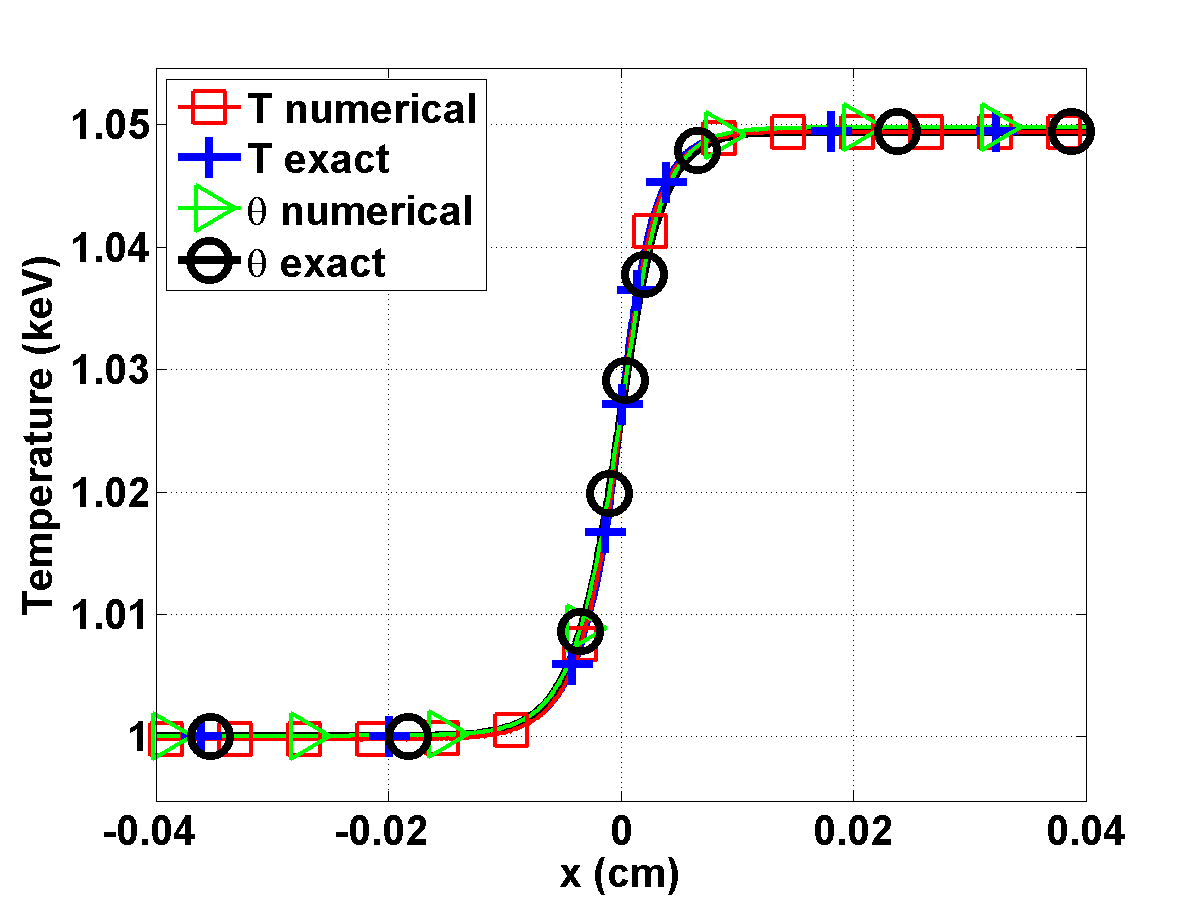
\includegraphics[width=\textwidth]{figs/Mach_1p05_nel_500_temperature.png}
        \caption{Material and radiation temperature profiles at steady state (Mach 1.05 test).}\label{fig:Mach105_temp}
\end{figure}
\begin{figure}[H]
                \centering
                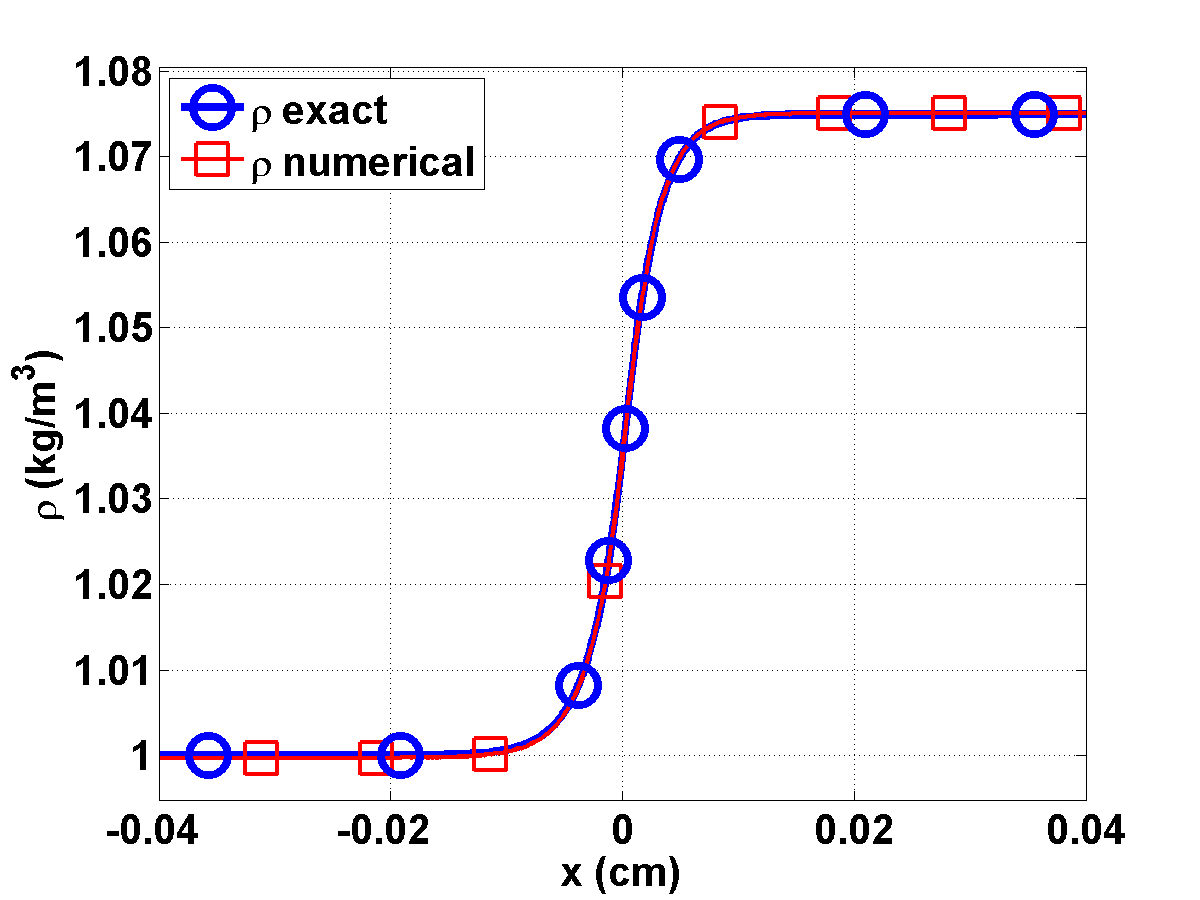
\includegraphics[width=\textwidth]{figs/Mach_1p05_nel_500_density}
        \caption{Material density profile at steady state (Mach 1.05 test).}\label{fig:Mach105_density}
\end{figure}
\begin{figure}[H]
                \centering
                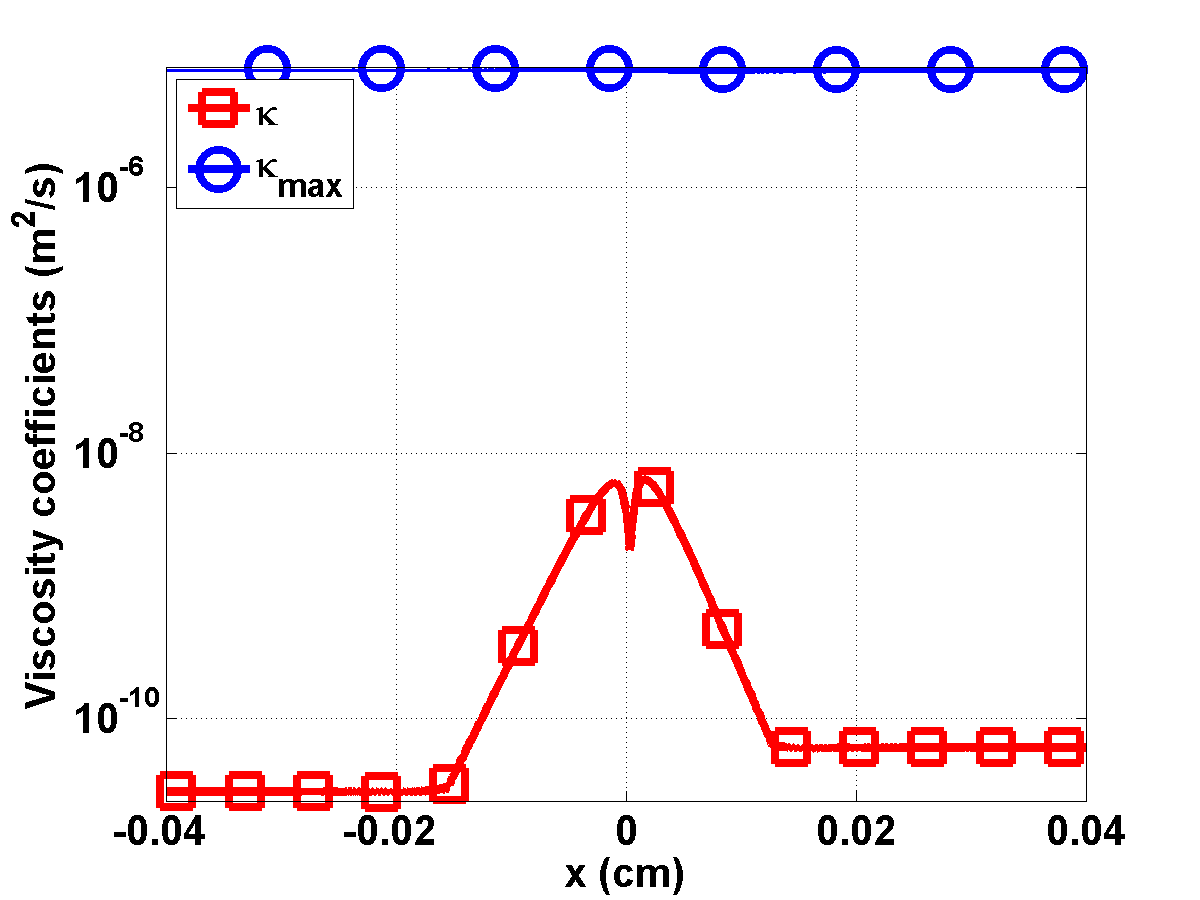
\includegraphics[width=\textwidth]{figs/Mach_1p05_nel_500_viscosity.png}
        \caption{First-order viscosity $\kappa_{max}$ and entropy viscosity $\kappa$ profiles at steady state for the Mach 1.05 test (logarithm scale).}\label{fig:Mach105_viscosity}
\end{figure}
The energy transfer between the material and radiation fields is not large enough to form a shock in the material. Thus, all of the material variables are smooth (\fig{fig:Mach105_temp} and \fig{fig:Mach105_density}) as well as the radiation temperature $\theta$. Because of the smoothness of the solution, the viscosity coefficient $\kappa$ is three order of magnitude smaller than the first-order viscosity coefficient $\kappa_{max}$ (\fig{fig:Mach105_viscosity}).

We also investigate the frozen in limit where the diffusion coefficient $D = \frac{c}{3\sigma_t}$ tends to zero by employing a very large value for the total opacity ($\sigma_t = 10^8 cm^{-1}$). The objective is to investigate whether the viscous regularization can efficiently stabilize the radiation equation when the physical diffusion term vanishes. The initial conditions and parameters are unchanged except for the total cross section that is now set to $10^8 cm^{-1}$. The simulation is run with three different spatial meshes (50, 100 and 200 spatial cells); the temperature, velocity, density, and, viscosity and diffusion coefficients profiles are plotted in \fig{fig:Mach_1p05_frozen_density}-\ref{fig:Mach_1p05_frozen_visc}.
%
\begin{figure}[H]
        \centering
        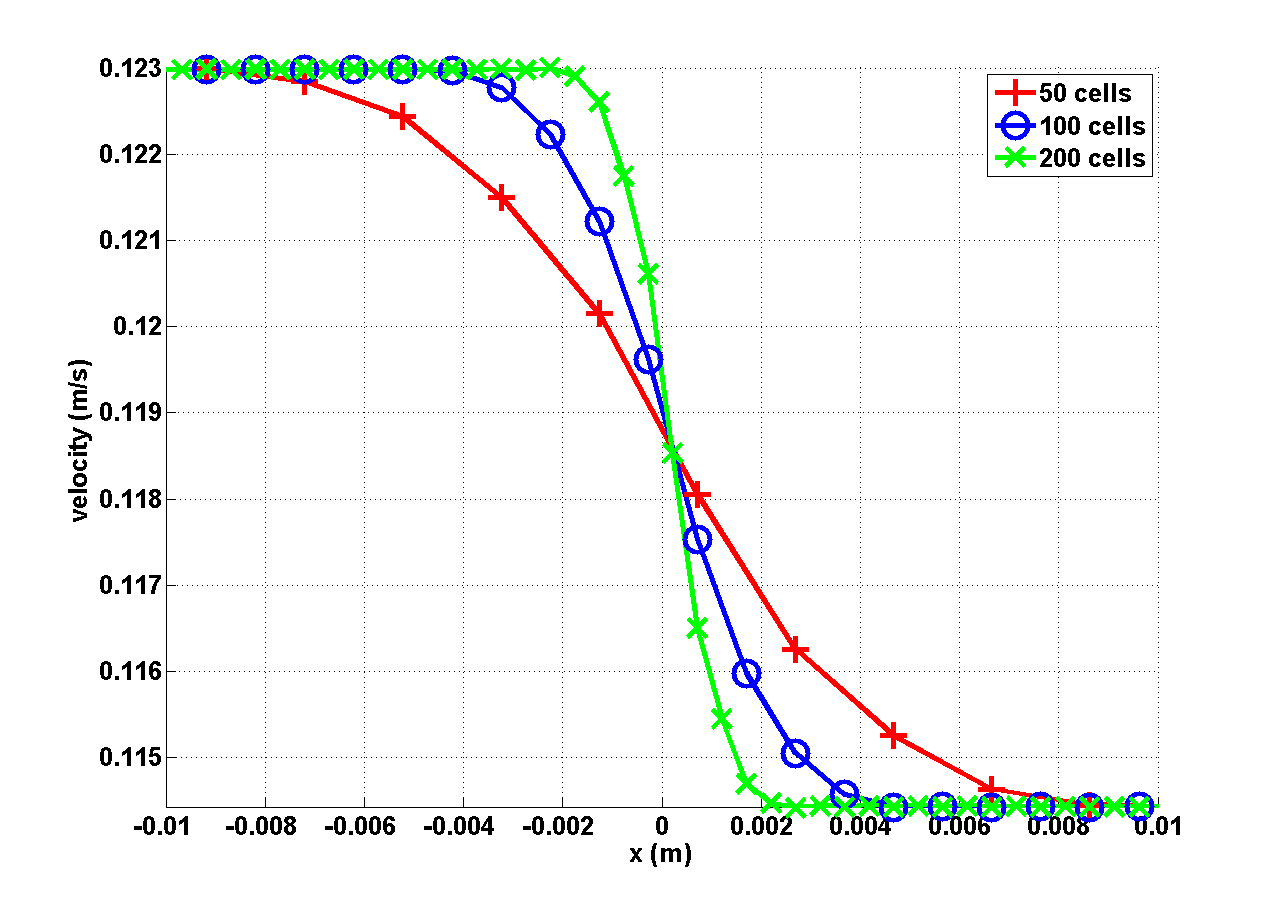
\includegraphics[width=\textwidth]{figs/Mach_1p05_zoom_in_velocity.png}
        \caption{Material velocity profile (Mach 1.05 test, zoom in the region of strong spatial variations).}
        \label{fig:Mach_1p05_frozen_density}
\end{figure}%
\begin{figure}[H]
            \centering
            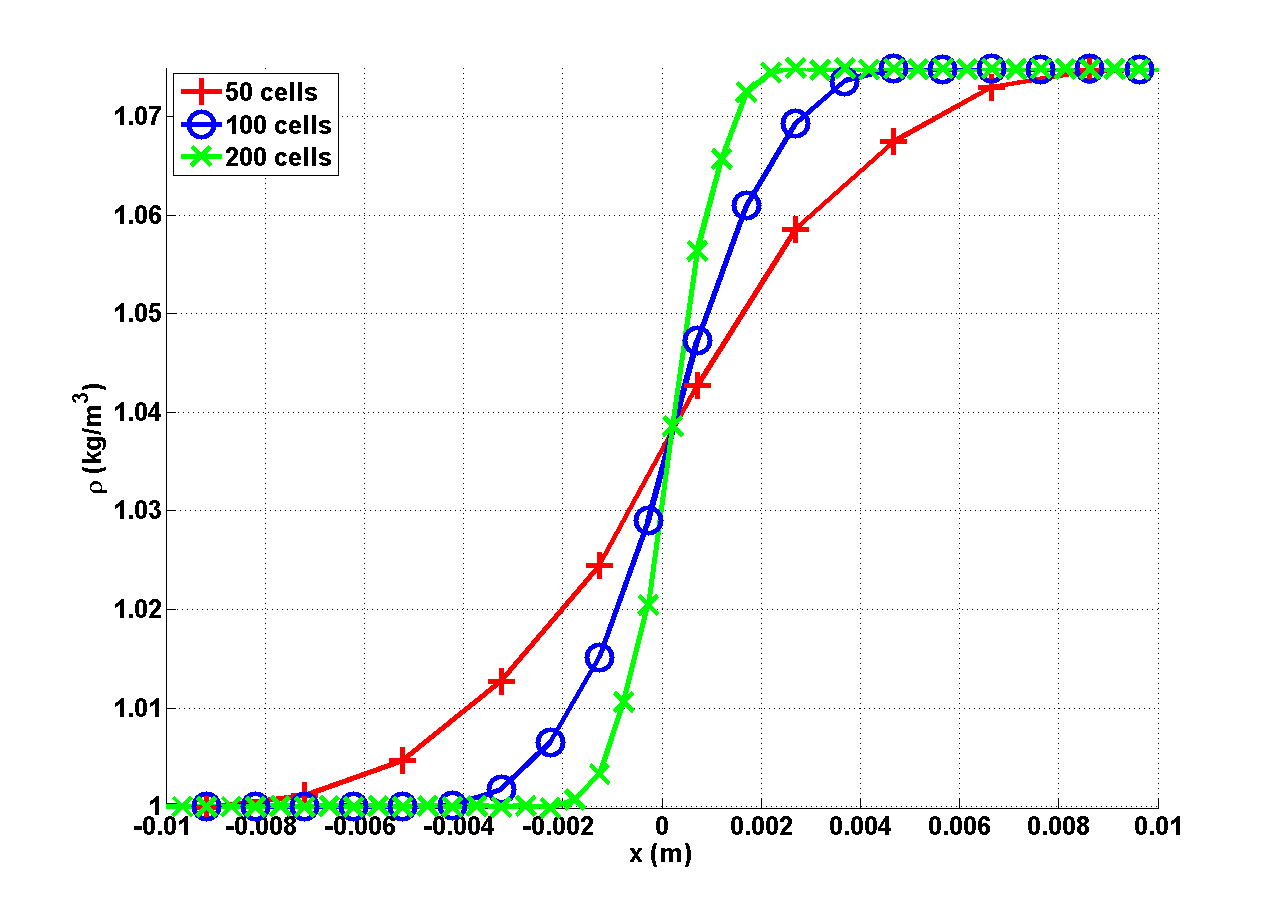
\includegraphics[width=\textwidth]{figs/Mach_1p05_zoom_in_density.png}
            \caption{Material density profile (Mach 1.05 test, zoom in the region of strong spatial variations).}
            \label{fig:Mach_1p05_frozen_velocity}
\end{figure}
\begin{figure}[H]
        \centering
        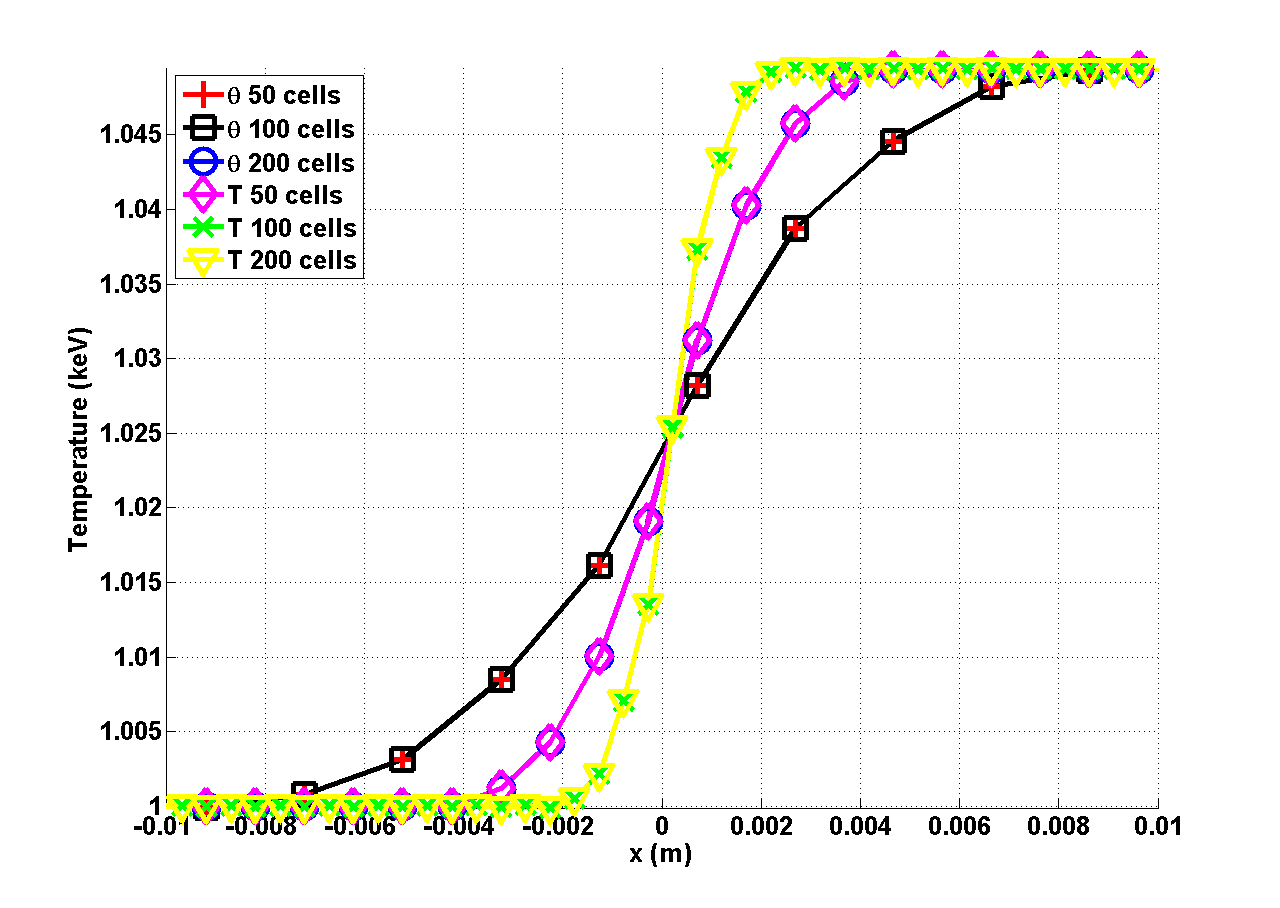
\includegraphics[width=\textwidth]{figs/Mach_1p05_zoom_in_temperatures.png}
        \caption{Material temperature profile (Mach 1.05 test, zoom in the region of strong spatial variation).}
        \label{fig:Mach_1p05_frozen_temp}
\end{figure}        
\begin{figure}[H]
        \centering
        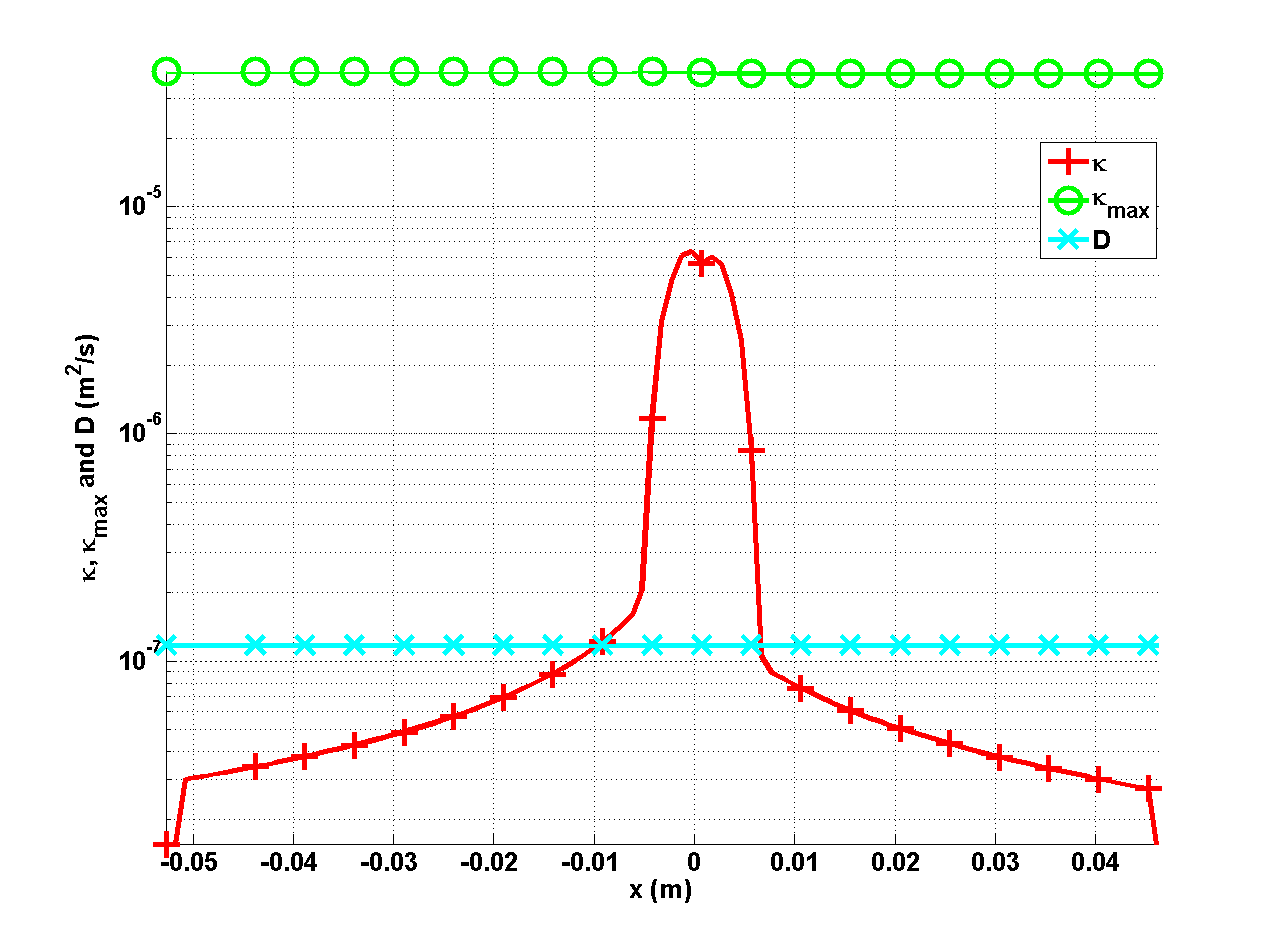
\includegraphics[width=\textwidth]{figs/Mach_1p05_frozen_in_viscosity_coeffs.png}
        \caption{Numerical viscosity and diffusion coefficients profiles with 100 spatial cells.}
        \label{fig:Mach_1p05_frozen_visc}
\end{figure}
%\caption{Solution profiles at steady-state for Mach 1.05 test in the frozen in limit.}\label{fig:1d_frozen_in}
%
The profiles presented in \fig{fig:Mach_1p05_frozen_density}-\ref{fig:Mach_1p05_frozen_temp} does not display any instability in the region of strong spatial variation
($x \in \left[ -0.1;\  0.1 \right]$). In \fig{fig:Mach_1p05_frozen_visc}, the viscosity coefficient is peaked but does not saturate to the first-order viscosity $\kappa_{max}$ (no shocks are present in that simulation). We note that the artificial viscosity value is always larger than the diffusion coefficient $D$ in the zone of strong variation; the viscous regularization efficiently stabilizes the radiation profile along with the material variables. Note that the viscosity coefficients $\kappa_{max}$ and $\kappa$ are defined proportional to the grid size and the square of the grid size, respectively, and thus will eventually become smaller than the diffusion coefficient as the mesh is refined. 

%%%%%%%%%%%%%%%%%%%%%%%%%%%%%%%%%%%%%%%%%%%%%%%%%%%%%%%%%%%%%
\subsubsection{A $1.2$ Mach hydrodynamic shock}
%%%%%%%%%%%%%%%%%%%%%%%%%%%%%%%%%%%%%%%%%%%%%%%%%%%%%%%%%%%%%

In this test, the material experiences a shock. The initial conditions, corresponding to a Mach number of $1.2$ at the inlet, are as follows: 
\begin{table}[H]
\caption{\label{tbl:table4} Initial conditions for Mach $1.2$.}
\begin{center}
\begin{tabular}{|c|c|c|}
\hline 
 & left  & right \\ \hline
$\rho$ $(g/cm^3)$ &$1.$ & $1.0749588$ \\ \hline
$u$ $(cm/sh)$& $0.1405588$ & $0.1083456$ \\ \hline
$T$ $(keV)$& $0.1$ & $0.1194751$\\ \hline
$\epsilon$ $(jerks/cm^3)$ & $1.372$ $10^{-6}$ & $2.7955320$ $10^{-6}$\\
\hline
\end{tabular}  
\end{center}  
\end{table}
The slab thickness is set to $L=0.045$ $cm$ and the initial step was located at $x_0 = 0$ $cm$. 
\begin{figure}[H]
       \centering
       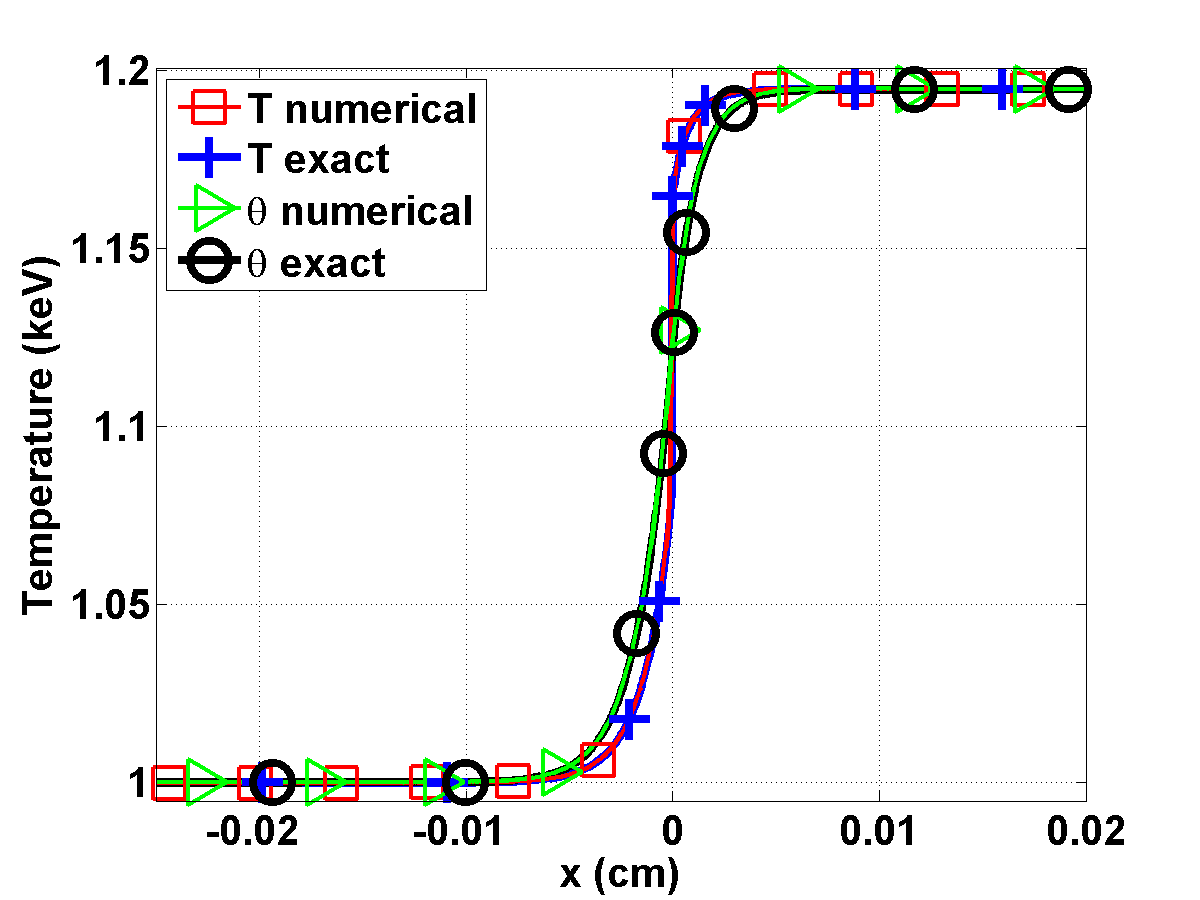
\includegraphics[width=\textwidth]{figs/Mach_1p2_nel_1000_temperature.png}
       \caption{Material and radiation temperature profiles at steady state (Mach 1.2 test).}\label{fig:Mach12_temp}
\end{figure}
The radiation and material temperatures have two different behaviors (\fig{fig:Mach12_temp}): the later experiences an embedded hydrodynamic shock, whereas the radiation temperature is smooth because of the diffusion term. The material temperature profile does not show any pre- and post-shock oscillations. In \fig{fig:Mach12_density}, the material density profile has a shock as well. The viscosity coefficient (\fig{fig:Mach12_viscosity}) is peaked in the shock as expected but does not saturate to the first-order viscosity. It is conjectured that the diffusion term in the radiation equation brings extra stability to the system. \\
Overall, the numerical solution behaves as expected in the shock and the entropy-based viscosity method seems to efficiently stabilize the numerical scheme.  
\begin{figure}[H]
                \centering
                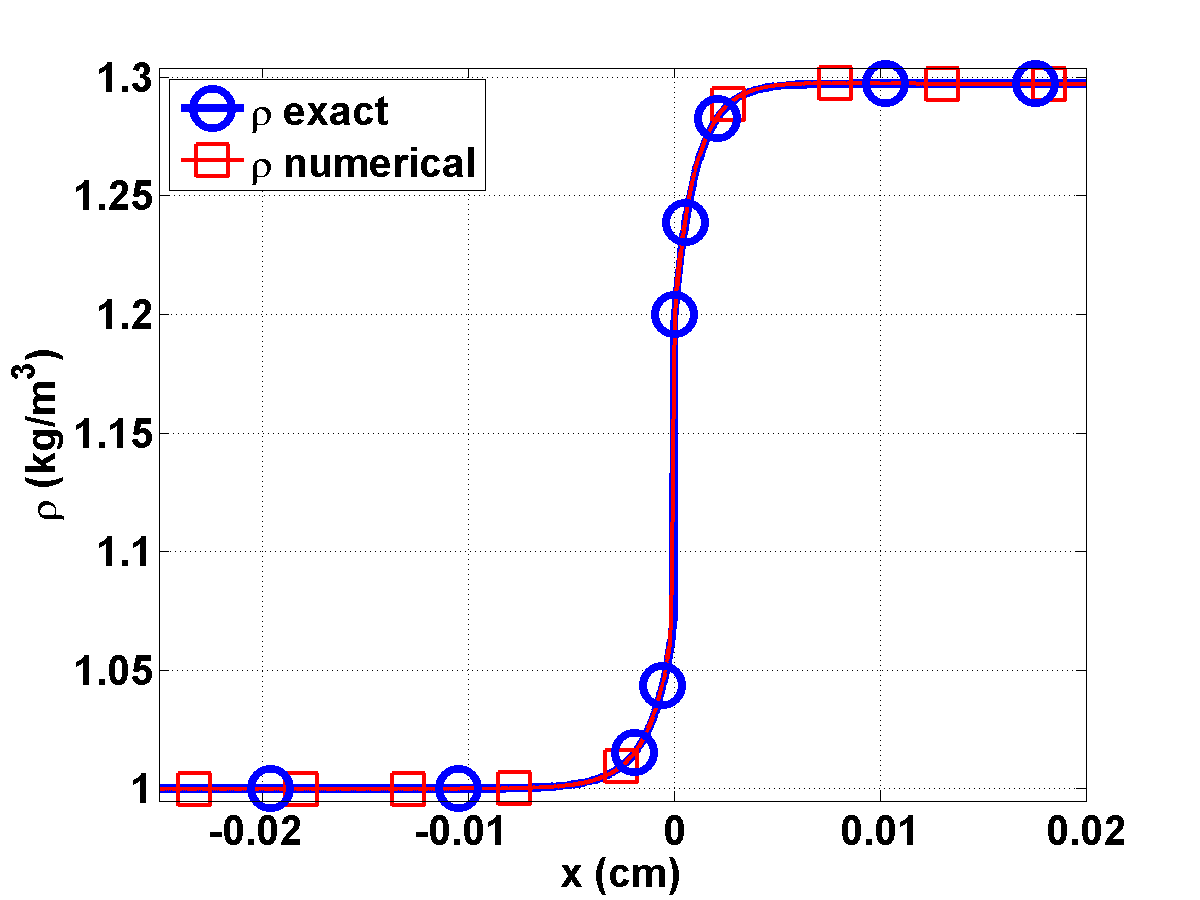
\includegraphics[width=\textwidth]{figs/Mach_1p2_nel_1000_density.png}
        \caption{Material density profile at steady state for Mach 1.2 test.}\label{fig:Mach12_density}
\end{figure}
\begin{figure}[H]
                \centering
                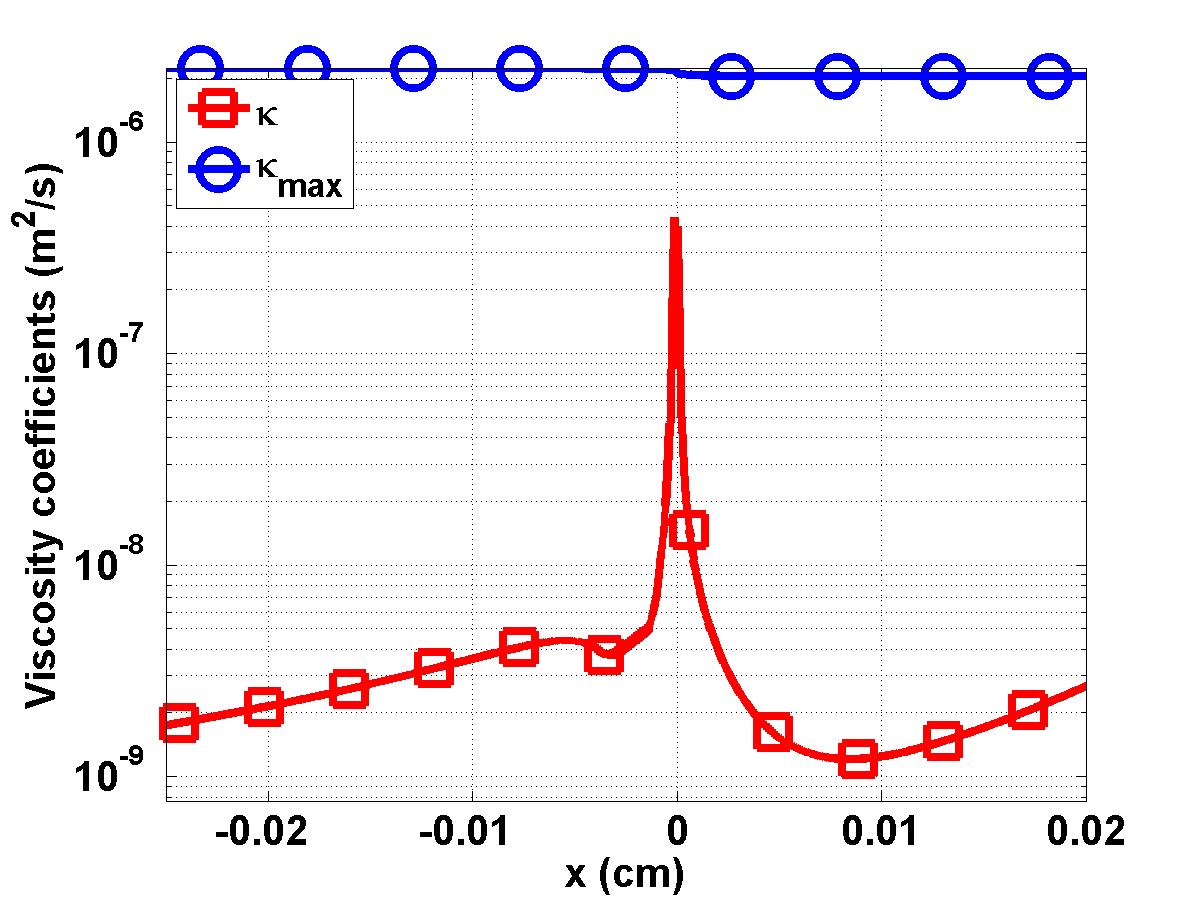
\includegraphics[width=\textwidth]{figs/Mach_1p2_nel_1000_viscosity.png}
        \caption{First-order viscosity $\kappa_{max}$ and entropy viscosity $\kappa_e$ profiles at steady state (Mach 1.2 test, logarithm scale).}\label{fig:Mach12_viscosity}
\end{figure}

%%%%%%%%%%%%%%%%%%%%%%%%%%%%%%%%%%%%%%%%%%%%%%%%%%%%%%%%%%%%%
\subsubsection{A Mach $2$ shock}
%%%%%%%%%%%%%%%%%%%%%%%%%%%%%%%%%%%%%%%%%%%%%%%%%%%%%%%%%%%%%

The Mach $2$ shock test has two features: a hydrodynamic shock and a Zeldovich spike, which make it interesting for testing the robustness of the entropy-based viscosity method. The initial conditions are specified in \tbl{tbl:table5} for a slab of length $L=0.04$ $cm$ with $x_0 = 0.$ $cm$.
\begin{table}[H]
\caption{\label{tbl:table5} Initial conditions for Mach $2$.}
\begin{center}
\begin{tabular}{|c|c|c|}
\hline 
 & left  & right \\ \hline
$\rho$ $(g/cm^3)$ &$1.$ & $1.0749588$ \\ \hline
$u$ $(cm/sh)$& $0.1405588$ & $0.1083456$ \\ \hline
$T$ $(keV)$& $0.1$ & $0.1194751$\\ \hline
$\epsilon$ $(jerks/cm^3)$ & $1.372$ $10^{-6}$ & $2.7955320$ $10^{-6}$\\
\hline
\end{tabular}  
\end{center}  
\end{table}
\begin{figure}[H]
                \centering
                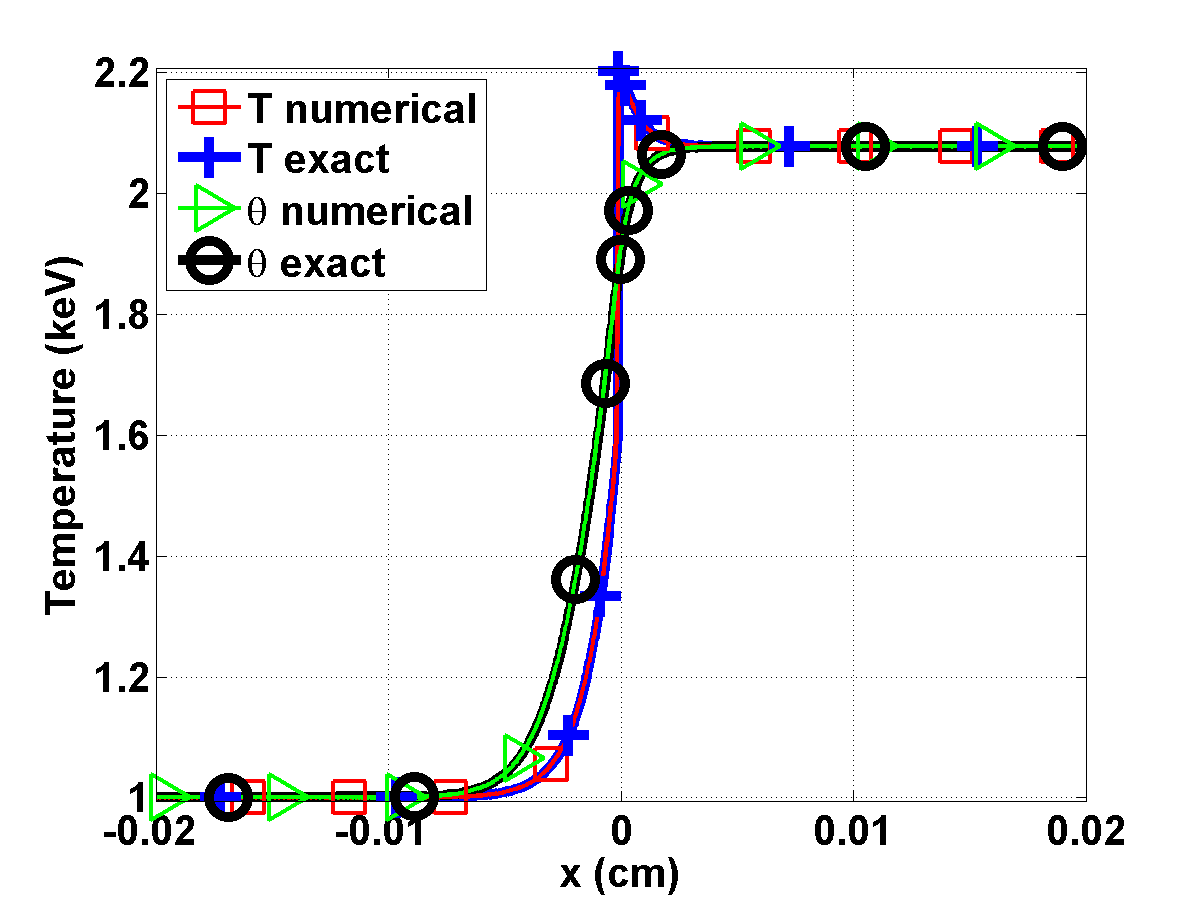
\includegraphics[width=\textwidth]{figs/Mach_2_nel_2000_temperature.png}
        \caption{Material and radiation temperature profiles at steady-state (Mach 2 test).}\label{fig:Mach2_temp}
\end{figure}
Once again, the radiation temperature profile is smooth and the material temperature experiences an embedded hydrodynamic shock and a peak as shown in \fig{fig:Mach2_temp}. In \fig{fig:Mach2_density}, the shock is well resolved. The viscosity coefficient profile is given in \fig{fig:Mach2_viscosity} and is peaked, once again, in the shock region. 

For comparison purpose, the same simulation was run with the first-order viscosity only, i.e., $\kappa$ was set equal to $\kappa_{max}$ for the whole domain in order to see the advantage of using a entropy viscosity coefficient. The results are given in \fig{fig:Mach2_tempEVandFO} for the material density and temperature. Numerical solutions with first- and entropy viscosity coefficients are graphed. The radiation temperature profile (not shown here) is not affected much by the first-order viscosity and the curves are coincident. This is expected because of the way the artificial viscosity term is treated in the radiation equation (\sect{sec:entropy-visc-meth}). However, on the same figure, the shock and peak in the material temperature profile are smoothed out: the shock is not as sharp and the peak amplitude is reduced because of the larger amount of viscosity added to the system. This test shows the benefits of using a high-order viscosity coefficient in order to avoid over-dissipation.
\begin{figure}[H]
                \centering
                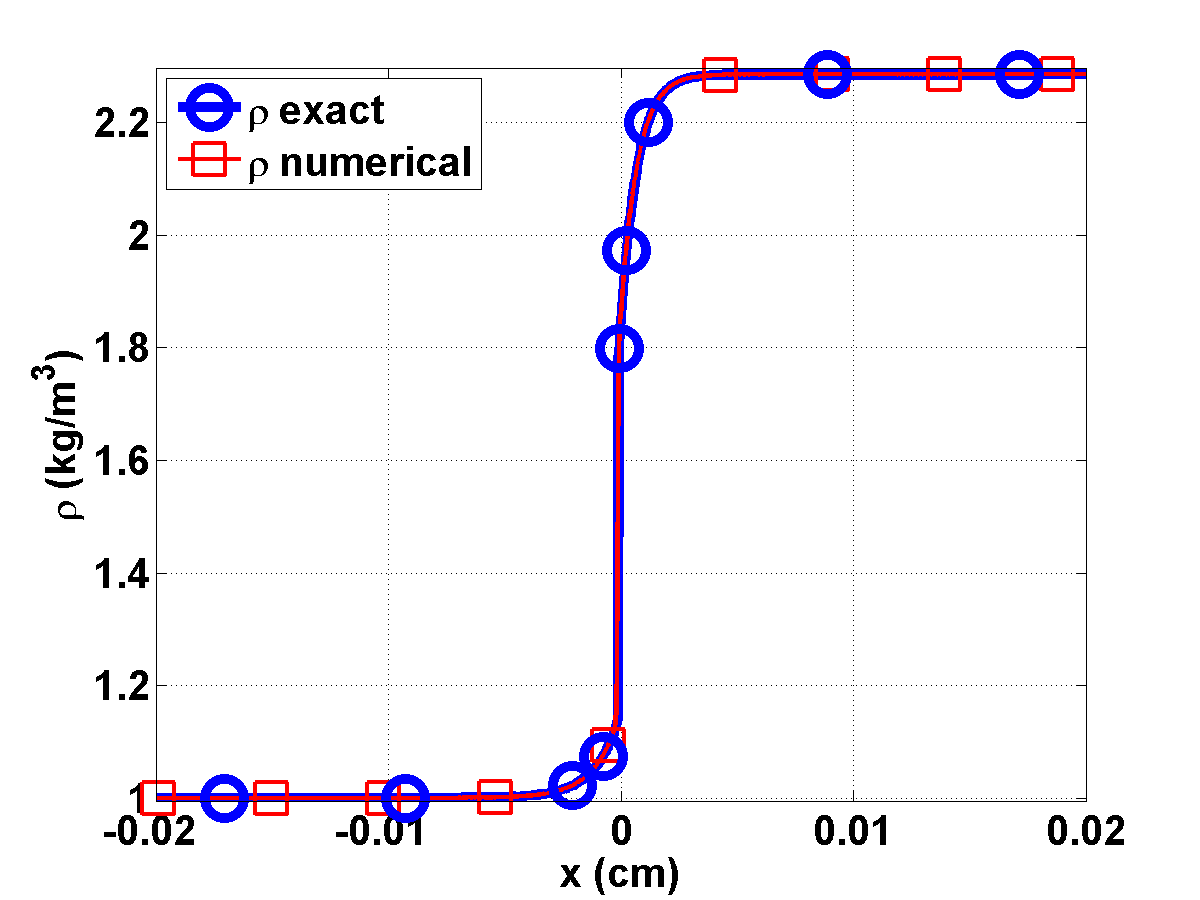
\includegraphics[width=\textwidth]{figs/Mach_2_nel_2000_density.png}
        \caption{Material density profile at steady-state (Mach 2 test).}\label{fig:Mach2_density}
\end{figure}
\begin{figure}[H]
                \centering
                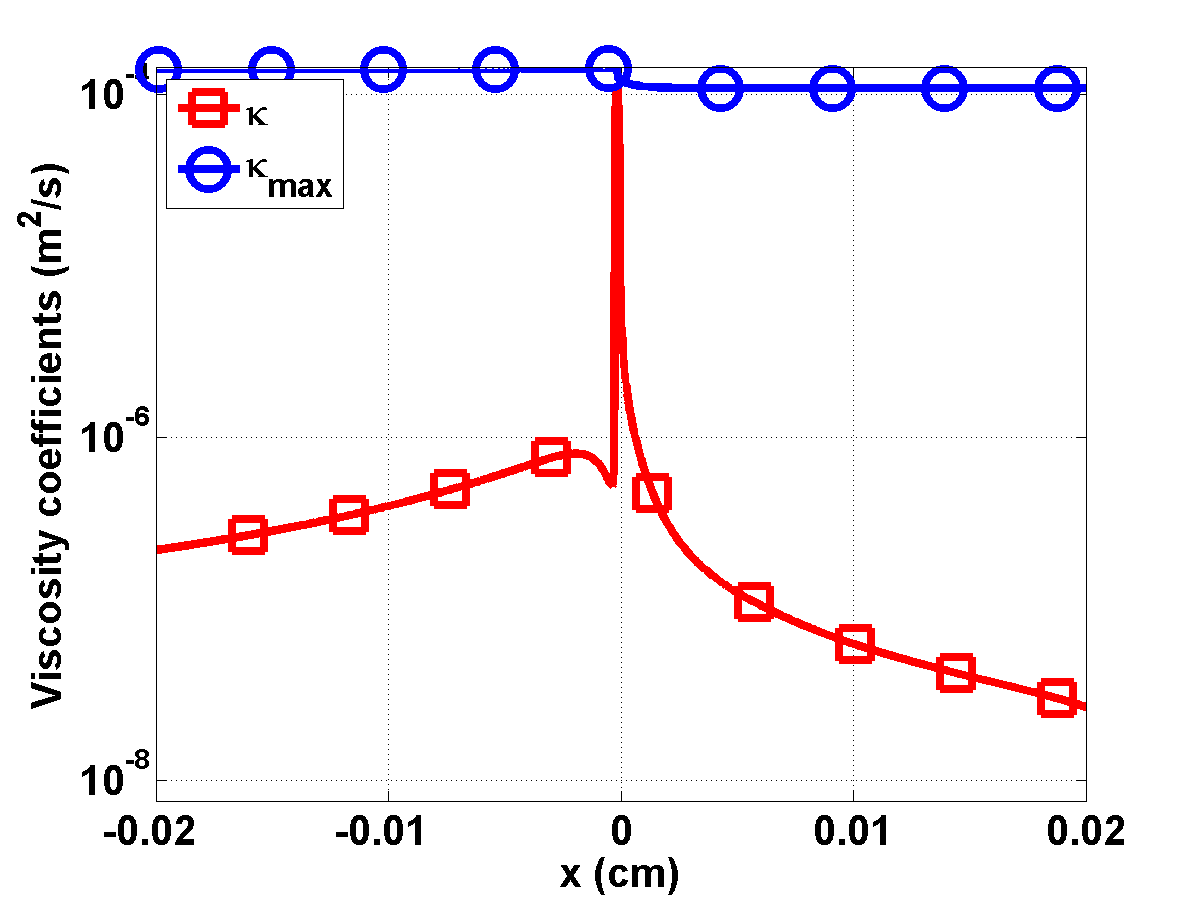
\includegraphics[width=\textwidth]{figs/Mach_2_nel_2000_viscosity.png}
        \caption{First-order viscosity $\kappa_{max}$ and entropy viscosity $\kappa$ profiles at steady state (Mach 2 test).}\label{fig:Mach2_viscosity}
\end{figure}
\begin{figure}[H]
                \centering
                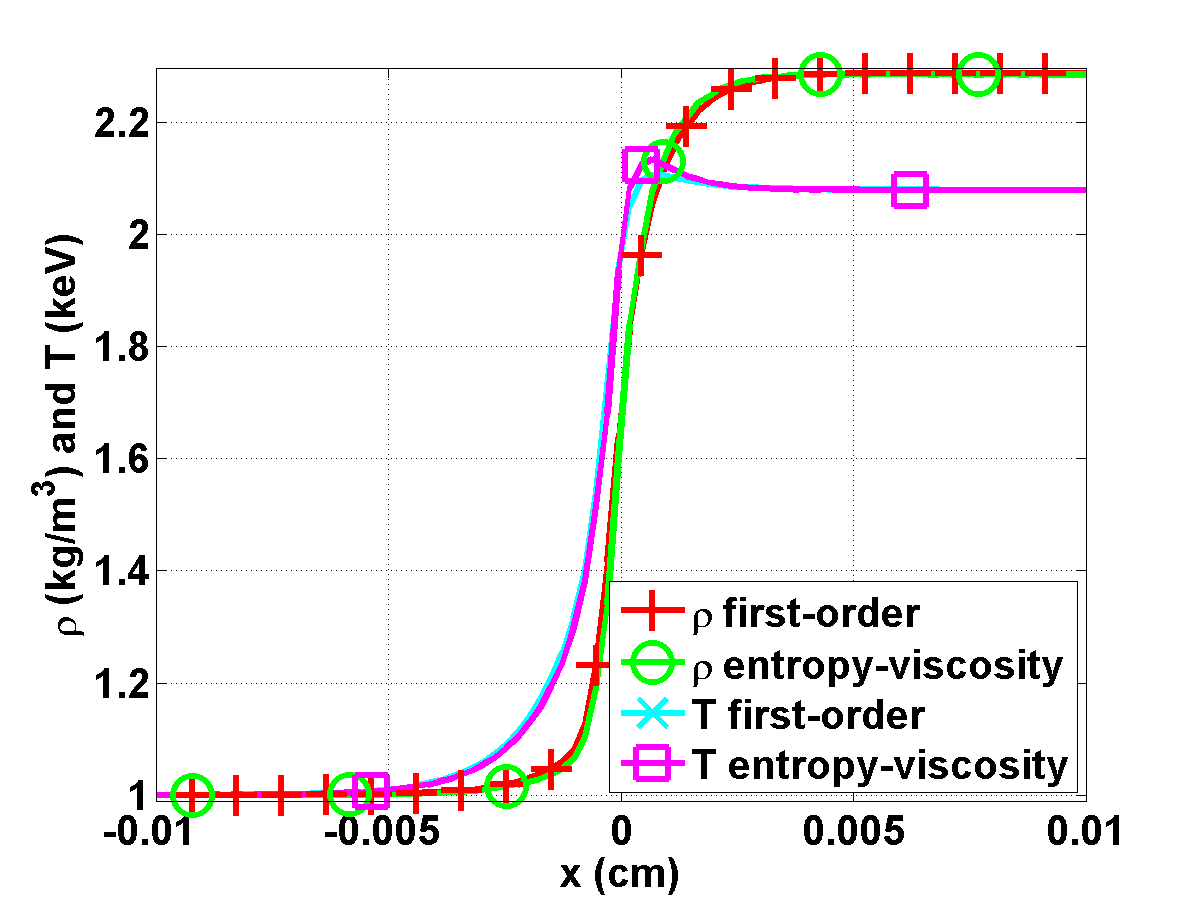
\includegraphics[width=\textwidth]{figs/Mach_2_fo_ev.png}
        \caption{Effect of the viscosity option on the material density and temperature profiles (Mach 2 test).}\label{fig:Mach2_tempEVandFO}
\end{figure}

%%%%%%%%%%%%%%%%%%%%%%%%%%%%%%%%%%%%%%%%%%%%%%%%%%%%%%%%%%%%%
\subsubsection{Mach $5$ shock}
%%%%%%%%%%%%%%%%%%%%%%%%%%%%%%%%%%%%%%%%%%%%%%%%%%%%%%%%%%%%%

A Mach $5$ test is run with the initial conditions of \tbl{tbl:table6} on a computational domain of length $L=0.05$ $cm$ ($x_0 = 0$ $cm$). Steady-state results are shown in \fig{fig:Mach5_temp}, \fig{fig:Mach5_density}, and \fig{fig:Mach5_viscosity} for the material and radiation temperatures, the density and the viscosity coefficients, respectively.
\begin{table}[H]
\caption{\label{tbl:table6} Initial conditions for Mach $5$.}
\begin{center}
\begin{tabular}{|c|c|c|}
\hline 
 & left  & right \\ \hline
$\rho$ $(g/cm^3)$ &$1.$ & $1.0749588$ \\ \hline
$u$ $(cm/sh)$& $0.1405588$ & $0.1083456$ \\ \hline
$T$ $(keV)$& $0.1$ & $0.1194751$\\ \hline
$\epsilon$ $(jerks/cm^3)$ & $1.372$ $10^{-6}$ & $2.7955320$ $10^{-6}$\\
\hline
\end{tabular}  
\end{center}  
\end{table}
\begin{figure}[H]
                \centering
                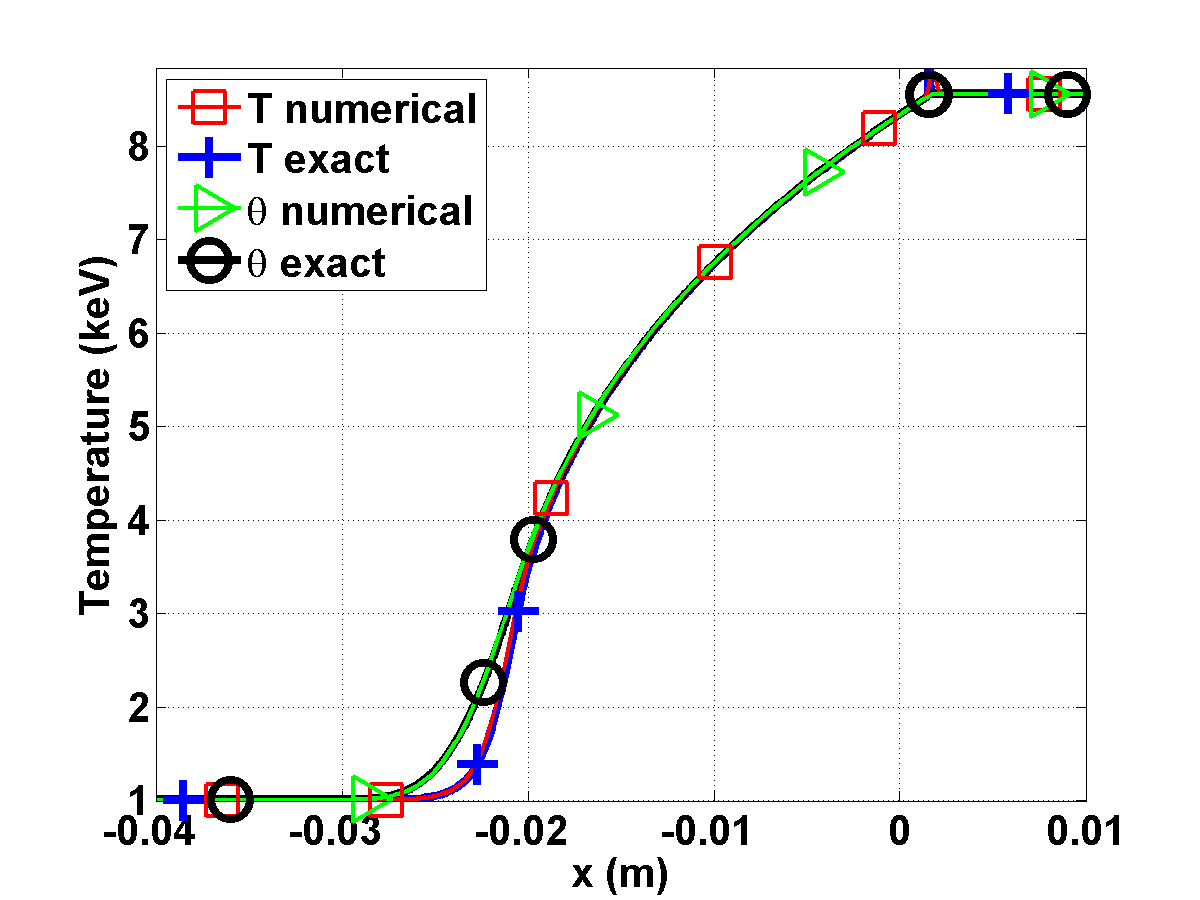
\includegraphics[width=\textwidth]{figs/Mach_5_nel_1000_temperature.png}
        \caption{Material and radiation temperature profiles at steady state for the Mach 5 test (zoom at the location of the peak).}\label{fig:Mach5_temp}
\end{figure}
\begin{figure}[H]
                \centering
                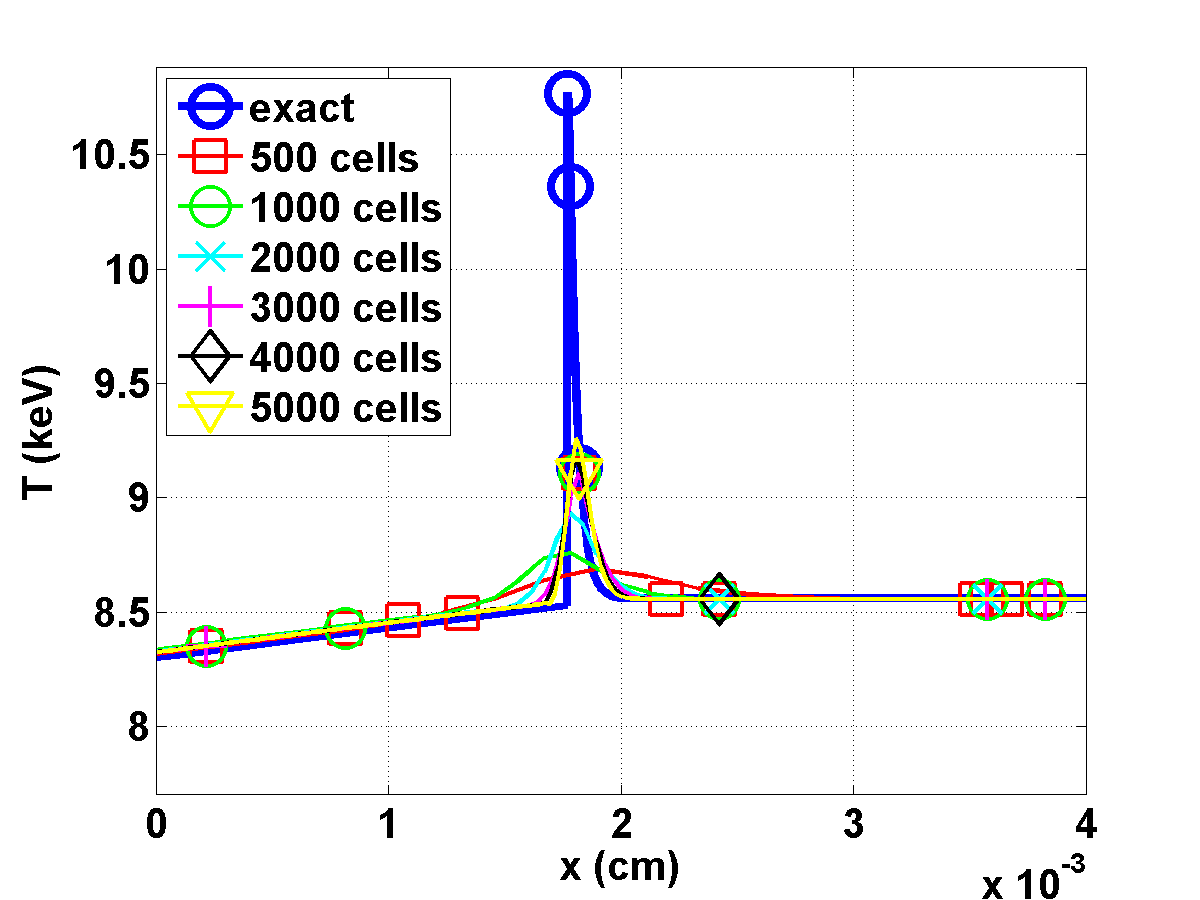
\includegraphics[width=\textwidth]{figs/Mach_5_comparison.png}
        \caption{Material temperature profiles at steady state for the Mach 5 test in the neighborhood of the spike.}\label{fig:Mach5_comparison}
\end{figure}
In \fig{fig:Mach5_temp}, the radiation temperature profile is smooth. The material temperature no longer exhibits an embedded hydrodynamic shock but shows a Zeldovich spike. The mesh with $500$ elements is not fine enough to correctly resolve the Zeldovich spike. In \fig{fig:Mach5_comparison}, the Zeldovich spike region is plotted for different mesh resolutions, using from $500$ to $5000$ elements: the peak is better resolved when using large numbers of elements and its position seems to be independent of the mesh size when appropriately refined. The density profile, \fig{fig:Mach5_density}, shows a shock located at the same position as the Zeldovich spike of the material temperature profile. The viscosity coefficient $\kappa$ is also peaked in the shock region, as expected. The material and radiation variables do not present any numerical oscillations. 
\begin{figure}[H]
                \centering
                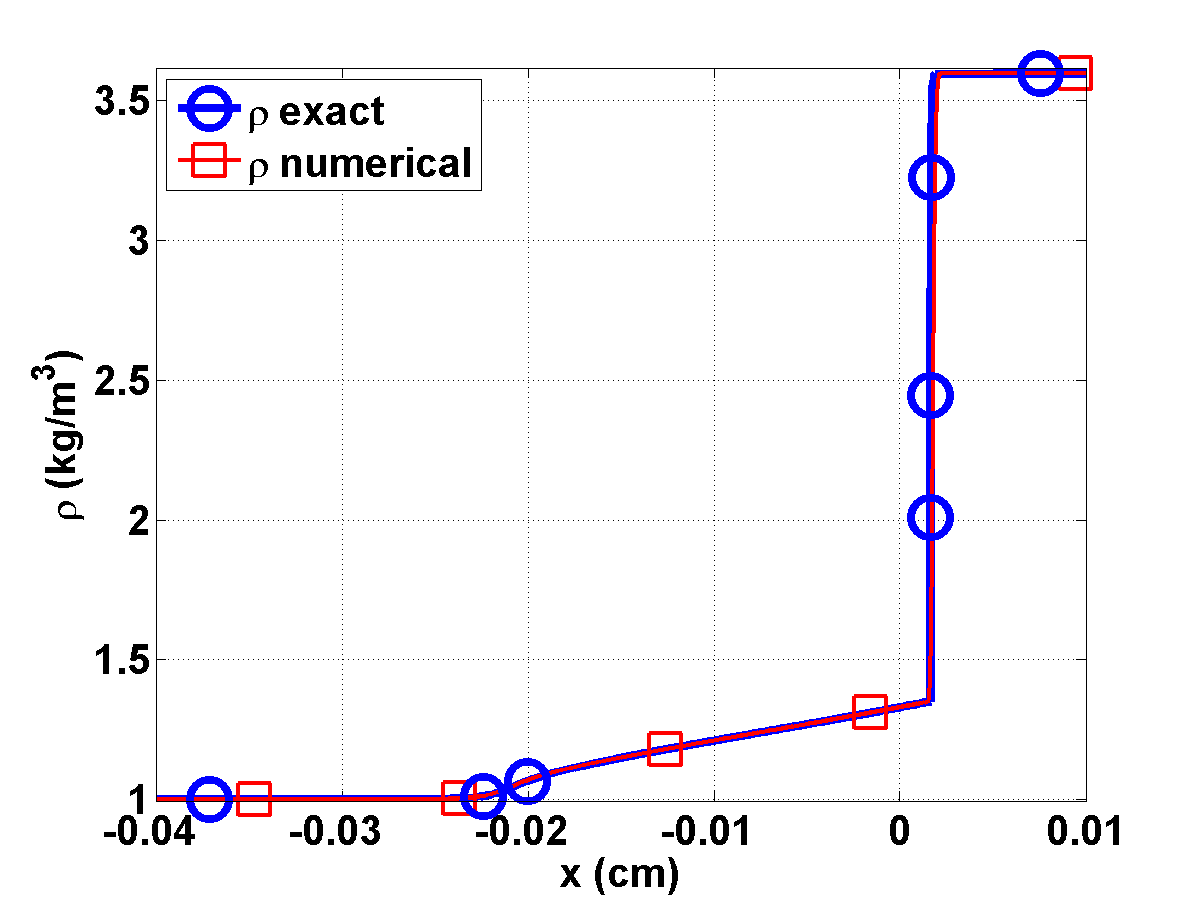
\includegraphics[width=\textwidth]{figs/Mach_5_nel_2000_density.png}
        \caption{Material density profile at steady state for the Mach 5 test.}\label{fig:Mach5_density}
\end{figure}
\begin{figure}[H]
                \centering
                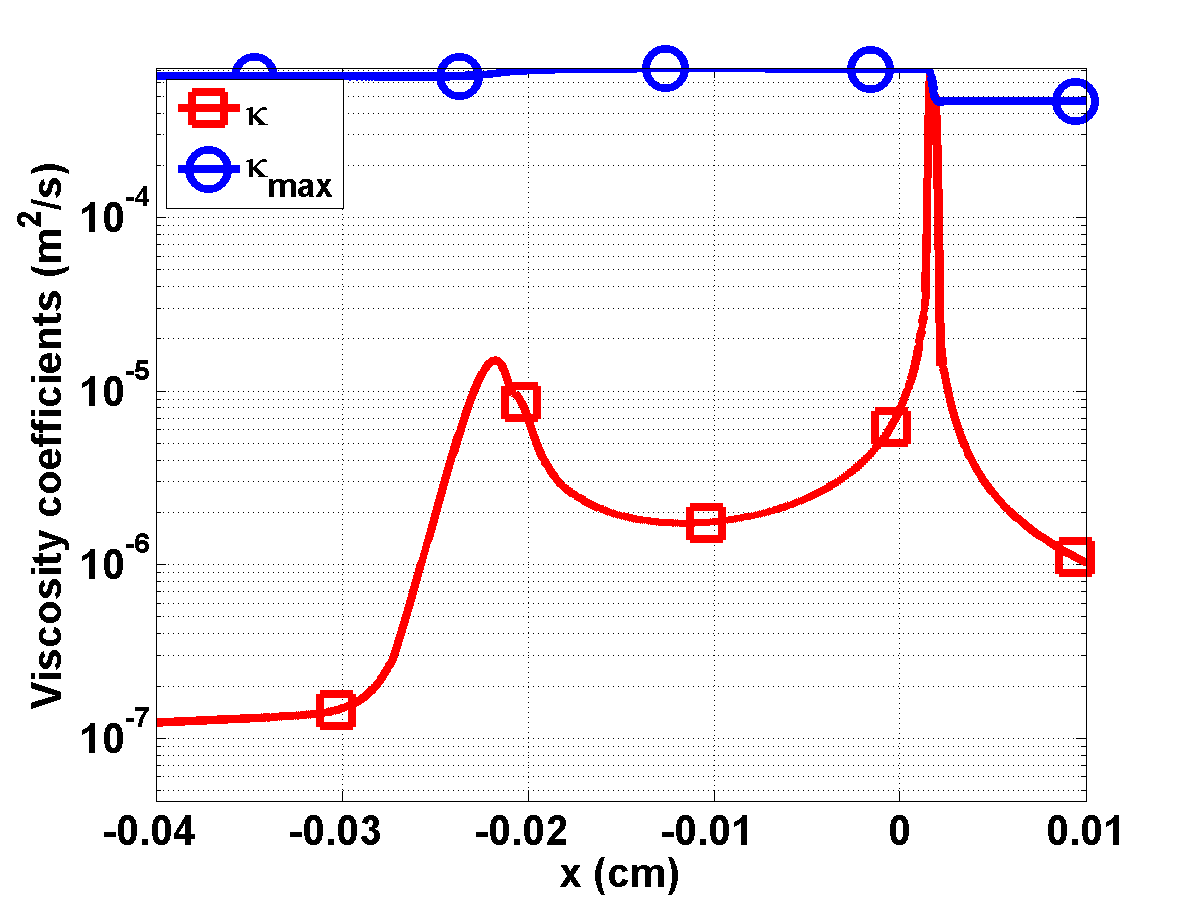
\includegraphics[width=\textwidth]{figs/Mach_5_nel_2000_viscosity.png}
        \caption{First-order viscosity $\kappa_{max}$ and entropy viscosity $\kappa_e$ profiles at steady state for the Mach 5 test.}\label{fig:Mach5_viscosity}
\end{figure}

%%%%%%%%%%%%%%%%%%%%%%%%%%%%%%%%%%%%%%%%%%%%%%%%%%%%%%%%%%%%%
\subsubsection{Mach $50$ shock} 
%%%%%%%%%%%%%%%%%%%%%%%%%%%%%%%%%%%%%%%%%%%%%%%%%%%%%%%%%%%%%

The Mach $50$ test is known to be challenging. The initial conditions are given in \tbl{tbl:table7}. The computational domain is of length $L=0.2$ $cm$. Results are once again given at steady state.
\begin{table}[H]
\caption{\label{tbl:table7} Initial conditions for Mach $50$.}
\begin{center}
\begin{tabular}{|c|c|c|}
\hline 
 & left  & right \\ \hline
$\rho$ $(g/cm^3)$ &$1.$ & $6.5189217$ \\ \hline
$u$ $(cm/sh)$& $585.6620$ & $89.84031$ \\ \hline
$T$ $(keV)$& $1.0$ & $85.51552$\\ \hline
$\epsilon$ $(jerks/cm^3)$ & $1.372$ $10^{-2}$ & $7.33726$ $10^{5}$\\
\hline
\end{tabular}  
\end{center}  
\end{table}
\begin{figure}[H]
                \centering
                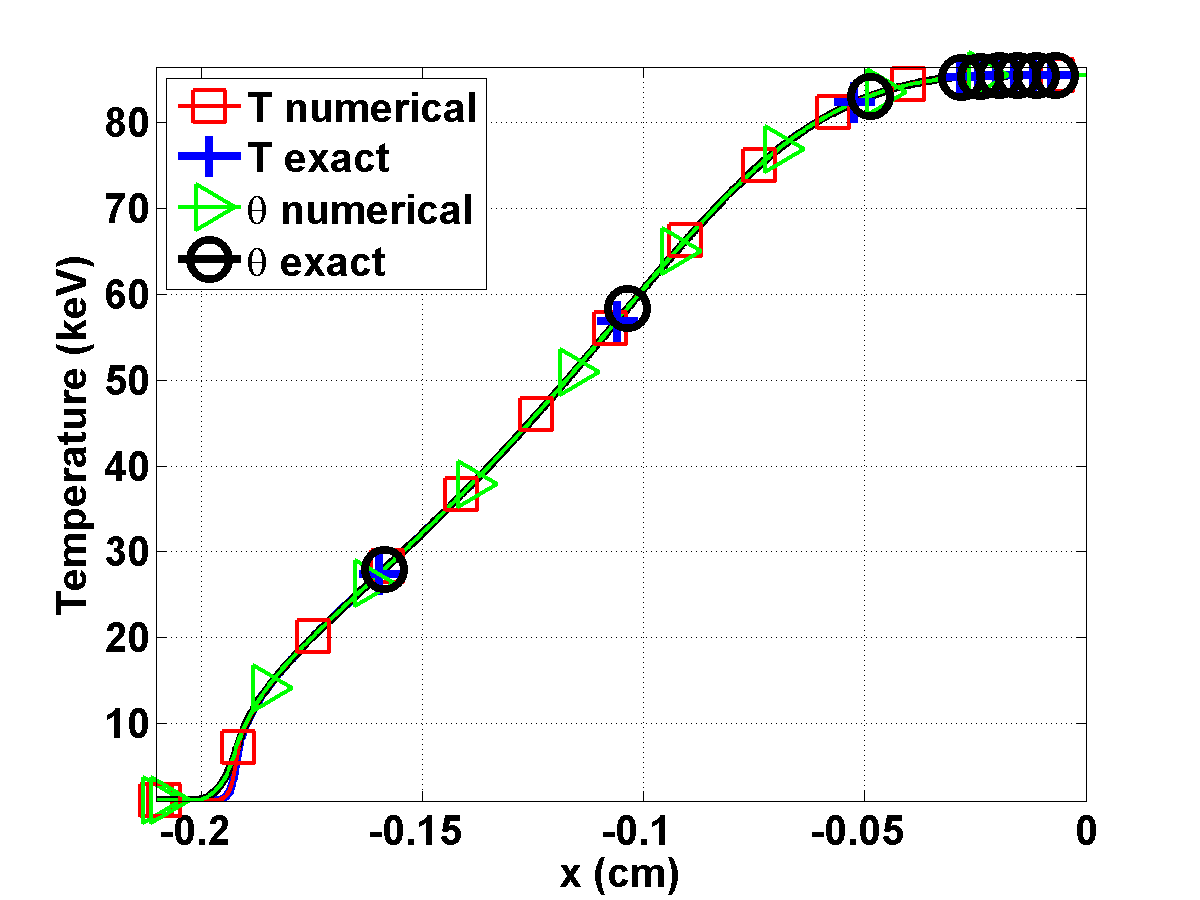
\includegraphics[width=\textwidth]{figs/Mach_50_nel_1000_temperature.png}
        \caption{Material and radiation temperature profiles at steady state for the Mach 50 test.}\label{fig:Mach50_temp}
\end{figure}
At Mach $50$, there is no embedded hydrodynamic shock forming as shown in \fig{fig:Mach50_temp}. The density profile is smooth as shown in \fig{fig:Mach50_density}. In \fig{fig:Mach50_temp}, the material and radiation temperatures overlap on all of the computational domain except for a small region located between $x=-0.2$ and $x=-0.18$ $cm$. In this particular region, the viscosity coefficient saturates to the first-order viscosity (see \fig{fig:Mach50_viscosity}) because of the inflection point in the material temperature profile. The artificial dissipative terms correctly stabilize the material temperature profile without altering the physical solution: the radiation temperature is expected to increase ahead of the material temperature.
\begin{figure}[H]
                \centering
                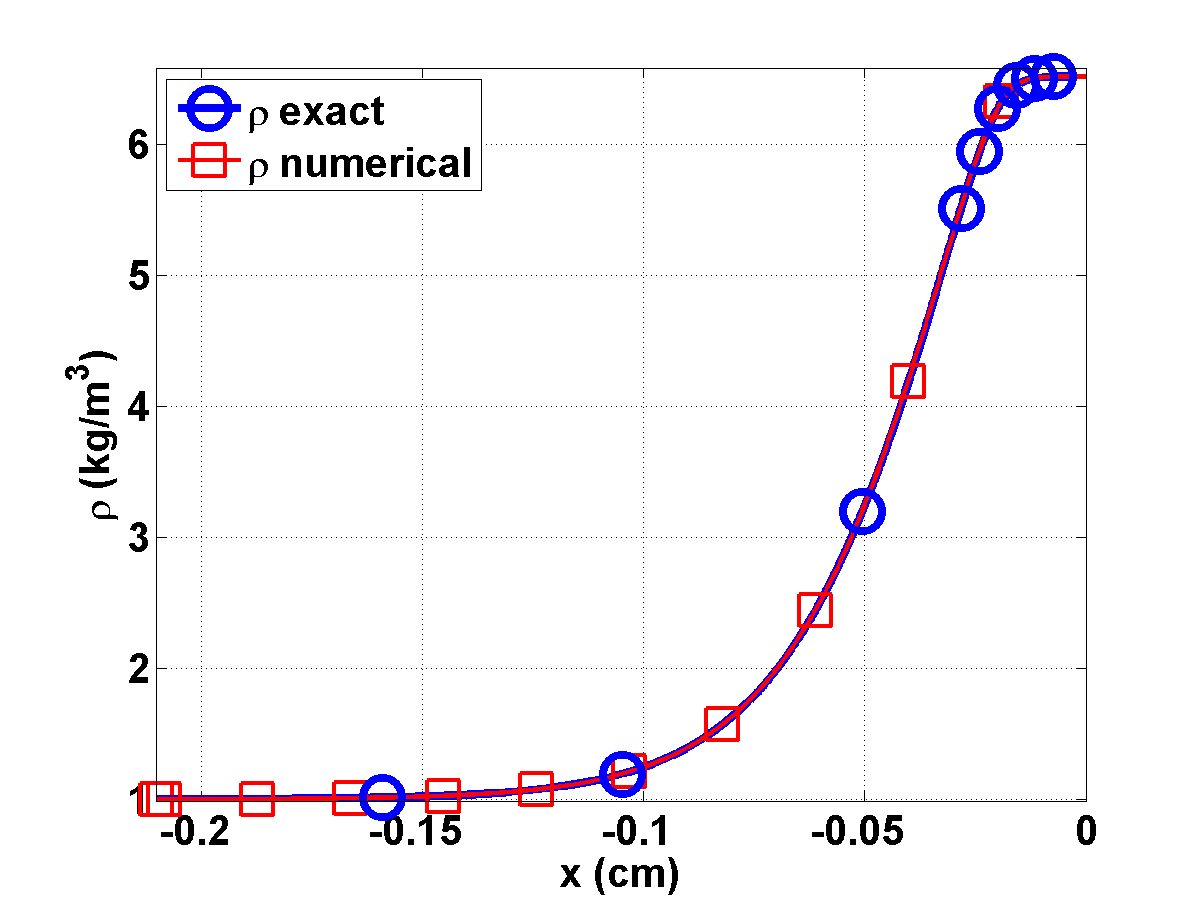
\includegraphics[width=\textwidth]{figs/Mach_50_nel_1000_density.png}
        \caption{Material density profile at steady-state for the Mach 50 test.}\label{fig:Mach50_density}
\end{figure}
\begin{figure}[H]
                \centering
                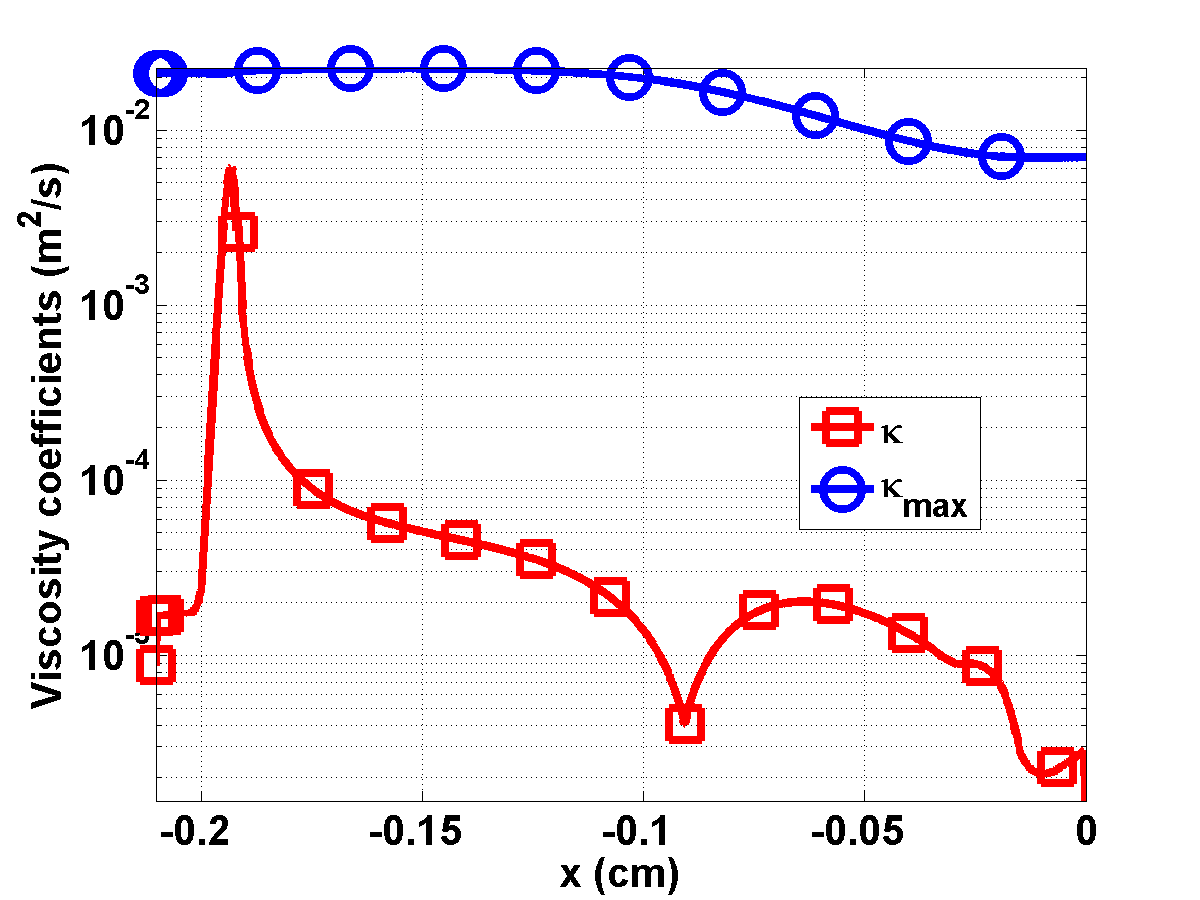
\includegraphics[width=\textwidth]{figs/Mach_50_nel_1000_viscosity.png}
        \caption{First-order viscosity $\kappa_{max}$ and entropy viscosity $\kappa_e$ profiles at steady-state for the Mach 50 test.}\label{fig:Mach50_viscosity}
\end{figure}

%%%%%%%%%%%%%%%%%%%%%%%%%%%%%%%%%%%%%%%%%%%%%%%%%%%%%%%%%%%%%
%%%%%%%%%%%%%%%%%%%%%%%%%%%%%%%%%%%%%%%%%%%%%%%%%%%%%%%%%%%%%
\section{Conclusions}
\label{sec:ccl}
%%%%%%%%%%%%%%%%%%%%%%%%%%%%%%%%%%%%%%%%%%%%%%%%%%%%%%%%%%%%%
%%%%%%%%%%%%%%%%%%%%%%%%%%%%%%%%%%%%%%%%%%%%%%%%%%%%%%%%%%%%%

The entropy viscosity method, an artificial viscosity shock-capturing technique, has been presented 
and applied to stabilize the 1-D non-equilibrium Grey Radiation-Hydrodynamic equations. 
We demonstrate that the viscous regularization terms of the entropy viscosity method are consistent with 
the entropy minimum principle and are valid for any equation of state with a concave entropy function. 
%
An asymptotic analysis shows that this viscous regularization preserves the equilibrium-diffusion limit 
and we recover equilibrium-diffusion results previously obtained in \cite{LowrieMorel} with a radiation-modified equation of state. 
Specifically, the viscous regularization of the non-equilibrium Grey Radiation-Hydrodynamic (GRH) equations 
is asymptotically equivalent to the viscous regularization of the equilibrium-diffusion limit (EDL) equation. 
Moreover, the entropy function derived for the GRH equations is proven to be asymptotically equivalent to 
the entropy function of the EDL equations.


%we have shown that the entropy-based viscosity method is a valid candidate for solving the 1-D Grey non-equilibrium Radiation-Hydrodynamic equations. A theoretical derivation is given for the derivation of a viscous regularization that is consistent with the entropy minimum principle and valid for all equation of states with a concave entropy function. 
%An asymptotic study showed that the viscous regularization conserves the equilibrium-diffusion limit and allows to recover the results initially obtained with the radiation-modified equation of state (REOS) \cite{LowrieMorel}. 

In the entropy viscosity method, the viscosity coefficient is defined proportionally to the entropy residual, measuring 
the local entropy production and thus enabling shock detection and tracking. 
%
Using manufactured solutions, we show second-order convergence rates for smooth solutions. The artificial dissipative terms do not affect the physical solution in the streaming and equilibrium-diffusion limits. 

Using standard radiation-hydrodynamic test cases with Mach numbers ranging from 1.05 to 50, we have shown that the entropy viscosity method behaves very satisfactorily. Physical features such as embedded hydrodynamic shocks and the Zeldovich spike are resolved accurately without spurious oscillations. The entropy viscosity coefficient is only peaked in the shock region and remains small elsewhere, as expected. 
%All of these results were obtained by using an unique definition of the viscosity coefficient that is computed on the fly. 
The addition of the viscous regularization terms to the set of equations is rather straightforward to implement in an existing code.

As future work, an extension to the multi-dimensional non-equilibrium grey radiation hydrodynamic equations is considered: all of the derivations presented in this paper hold in higher dimensions (the definitions for the viscous regularization fluxes and the viscosity coefficients need not to be modified). Furthermore, it can be of interest to model the radiation equation with an $S_n$ transport approximation and to apply the entropy-based artificial viscosity to the resultant radiation-hydrodynamics equations. 
% Given the advective nature of the $S_n$ equations, numerical stabilization would need to be added to these equations as well.

%%%%%%%%%%%%%%%%%%%%%%%%%%%%%%%%%%%%%%%%%%%%%%%%%%%%%%%%%%%%%
%%%%%%%%%%%%%%%%%%%%%%%%%%%%%%%%%%%%%%%%%%%%%%%%%%%%%%%%%%%%%
\section*{Acknowledgments}
The authors would like to acknowledge Jim Ferguson for providing the semi-analytical solutions and Bojan Popov for many fruitful discussions. 
%%%%%%%%%%%%%%%%%%%%%%%%%%%%%%%%%%%%%%%%%%%%%%%%%%%%%%%%%%%%%
%%%%%%%%%%%%%%%%%%%%%%%%%%%%%%%%%%%%%%%%%%%%%%%%%%%%%%%%%%%%%

\newpage
\begin{appendices}
%%%%%%%%%%%%%%%%%%%%%%%%%%%%%%%%%%%%%%%%%%%%%%%%%%%%%%%%%%%%%
%%%%%%%%%%%%%%%%%%%%%%%%%%%%%%%%%%%%%%%%%%%%%%%%%%%%%%%%%%%%%
\section{Proof of the entropy minimum principle for the Radiation-Hydrodynamic equations with viscous regularization}
\label{app:appendixA}
%%%%%%%%%%%%%%%%%%%%%%%%%%%%%%%%%%%%%%%%%%%%%%%%%%%%%%%%%%%%%
%%%%%%%%%%%%%%%%%%%%%%%%%%%%%%%%%%%%%%%%%%%%%%%%%%%%%%%%%%%%%

In this appendix, a demonstration of the entropy minimum principle for the system of equations \eqt{eq:regularized_hyperbolic_GRH} is given (the demonstration is carried out for the 1-D version of the equations and can easily be generalized to multiple dimensions). This proof, inspired by \cite{jlg}, details the steps that lead to the derivation of the dissipative terms for the GRH equations based on the entropy minimum principle.\\
We start with the hyperbolic system given in \eqt{eq:GRH_hyperbolic} and add dissipative terms to each equation as follows:
\begin{equation}
\label{eq:app_equ1bis}
\left\{
\begin{array}{llll}
\partial_t (\rho  ) + \partial_x (\rho u)  = \partial_x f \\
\partial_t (\rho u) + \partial_x \left(\rho u^2 +  P + \frac{\epsilon}{3} \right) = \partial_x g  \\
\partial_t (\rho E) + \partial_x \left[ u \left( \rho E +P \right) \right] + \frac{u}{3} \partial_x \epsilon = \partial_x \left( h + ug \right) \\
\partial_t \epsilon + u \partial_x \epsilon + \frac{4}{3} \epsilon \partial_x u = \partial_x l
\end{array}
\right. \,,
\end{equation}
where $f$, $g$, $h$ and $l$ are dissipative terms to be determined.
\eqt{eq:app_equ1bis} is then recast as a function of the primitive variables $(\rho, u, e, \epsilon)$ to yield:
\begin{equation}
\label{eq:app_equ1}
\left\{
\begin{array}{llll}
\frac{D \rho}{Dt} + \rho \partial_x u = \partial_x f \\
\rho \frac{Du}{Dt} + \partial_x \left( P + \frac{\epsilon}{3} \right) = \partial_x g - u \partial_x f  \\
\rho \frac{De}{Dt} + P \partial_x u = \partial_x h + g \partial_x u + \left( 0.5 u^2 - e \right) \partial_x f \\
\frac{D\epsilon}{Dt} + \frac{4}{3} \epsilon \partial_x u = \partial_x l
\end{array}
\right. 
\end{equation}
where we recall that $\matder{(\cdot)} = \partial_t (\cdot) + u \partial_x (\cdot)$. 
The right-hand side of the internal energy equation can be simplified by choosing the dissipative terms $g$ and $h$ as follows: $h = \tilde{h} -0.5 u^2 f$ and $g = \rho \mu \partial_x u + uf$ where $\mu \geq 0$ is a viscosity coefficient. Using these definitions, the system of equations given in \eqt{eq:app_equ1} becomes:
\begin{equation}
\label{eq:app_equ1ter}
\left\{
\begin{array}{llll}
\frac{D \rho}{Dt} + \rho \partial_x u = \partial_x f \\
\rho \frac{Du}{Dt} + \partial_x \left( P + \frac{\epsilon}{3} \right) = \partial_x g - u \partial_x f  \\
\rho \frac{De}{Dt} + P \partial_x u = \rho \mu (\partial_x u)^2 + \partial_x \tilde{h} - e \partial_x f \\
\frac{D\epsilon}{Dt} + \frac{4}{3} \epsilon \partial_x u = \partial_x l
\end{array}
\right. \,.
\end{equation}
This system of equations admits an entropy function $s$ that depends on density $\rho$, internal energy $e$, and radiation energy density $\epsilon$. In order to prove the entropy minimum principle, a conservation statement satisfied by the entropy is needed. This equation which is referred to as the entropy residual $D_e(x,t)$, can be obtained by a combination of the equations given in \eqt{eq:app_equ1ter}. This process is motivated by the following (chain rule) 
\begin{equation}
\label{eq:app_equ2}
\partial_{\alpha} s = \partial_{\rho} s \partial_{\alpha} \rho +  \partial_{e} s \partial_{\alpha}e +  \partial_{\epsilon} s \partial_{\alpha} \epsilon \text{,}
\end{equation}
 which holds for any independent variable $\alpha=x,t$. We introduce the following viscous fluxes:
 \begin{equation}
 \left\{
 \begin{array}{ccc}
f &= \kappa \partial_x \rho \\
\tilde{h} &= \kappa \partial_x (\rho e) \\
l &= \kappa \partial_x \epsilon
 \end{array}
 \right. \,,
 \end{equation}
 where $\kappa$ is another positive viscosity coefficient. \\
 Thus, using the continuity, internal energy, and radiation equations of \eqt{eq:app_equ1ter} and the relationship \eqt{eq:app_equ2}, the following conservation statement satisfied by the entropy $s$ is obtained:
 \begin{multline}
 \label{eq:app_entr_eq_non_equil}
\rho \frac{Ds}{Dt} = - \underbrace{\left( P \partial_e s + \rho^2 \partial_{\rho} s + \frac{4}{3} \rho \epsilon \partial_{\epsilon} s \right) \partial_x u}_\textrm{(a)} + \partial_x \left( \rho \kappa \partial_x s \right) + \kappa \partial_x \rho \partial_x s \\- \rho \kappa \underbrace{X A X^T}_\textrm{(b)} + \underbrace{ s_e \rho \mu (\partial_x u)^2}_\textrm{(c)} \,,
 \end{multline} 
 where $X$ is a row vector defined as $X=\left( \partial_x \rho, \partial_x e, \partial_x \epsilon \right)$ and $A$ is the $3 \times 3$ symmetric matrix
 \begin{equation}
 A = 
 \left[
 \begin{array}{ccc}
\rho^{-2}\partial_{\rho} \left( \rho^2 \partial_{\rho} s \right) & \partial_{\rho,e} s & \partial_{\rho} \left( \rho \partial_{\epsilon} s \right) \\
 \partial_{\rho,e} s & \partial_{e,e} s & \partial_{e,\epsilon} s \\
 \partial_{\rho} \left( \rho \partial_{\epsilon} s \right) & \partial_{e,\epsilon} s & \partial_{\epsilon,\epsilon} s
 \end{array}
 \right] .
 \end{equation}
 In order to show that the entropy minimum principle holds, the signs of the terms $(a)$, $(b)$ and $(c)$ in \eqt{eq:app_entr_eq_non_equil} need to be studied.\\
Regarding term $(a)$, we assume that $P \partial_e s + \rho^2 \partial_{\rho} s + \frac{4}{3} \rho \epsilon \partial_{\epsilon} s=0$. The motivation for this is two-fold. First, for term $(a)$ to always be positive would require that $P \partial_e s + \rho^2 \partial_{\rho} s + \frac{4}{3} \rho \epsilon \partial_{\epsilon} s$ be constantly of the opposite sign of $\partial_x u$; however, the thermodynamic variables cannot be a function of the material velocity or its derivative under a non-relativistic assumption. 
% Such a statement would not be true when dealing with relativistic equations of state. 
Second, a similar relationship, $P \partial_e s + \rho^2 \partial_{\rho} s = 0$, holds for the standard Euler equations (i.e., without the radiation energy); see \cite{jlg}. \\
The term $(b)$, $XAX^T$, is a quadratic form and its sign is determined by looking at the positiveness of matrix $A$ \cite{Evans}. Here we need to prove that $A$ is negative-definite which is equivalent to showing the three following inequalities:
\begin{equation}
 \left\{
 \begin{array}{ccc}
 A_1 \geq 0 \\
 A_2 \leq 0 \\
 A_3 = A \geq 0
 \end{array}
 \right. \,,
 \end{equation}
 where $A_k$ is the $k^{th}$ order leading principle minor. Determining the sign of the last inequality that corresponds to the determinant of the $3$ by $3$ matrix $A$ can be difficult and needs to be simplified. Zeroing out the off-diagonal entries of the last row or column would simplify the expression for the determinant of $A$. This can be achieved by assuming $\partial_{\rho}(\rho \partial_{\epsilon} s)$ and $\partial_{e, \epsilon} s$ are zero, which requires the following form for the entropy function:
\begin{equation}
\label{eq:app_equ4}
s(\rho, e, \epsilon) = s_{Euler}(\rho,e) + s_{rad}(\rho, \epsilon) = s_{Euler}(\rho,e) + \frac{\rho^{(0)}}{\rho}\tilde{s}_{rad}(\epsilon) \text{. } 
\end{equation}
where $s_{Euler}$ and $\tilde{s}_{rad}$ are two functions whose properties will be provided later, and $\rho^{(0)}$ is a constant of same units as density and is assumed positive to ensure positivity of $s(\rho,e,\epsilon)$.
Next, using the expression of the entropy given in \eqt{eq:app_equ4}, matrix $A$ becomes:
 \begin{equation}
 A = 
 \left[
 \begin{array}{ccc}
\partial_{\rho} \left( \rho^2 \partial_{\rho} s_{Euler} \right) & \partial_{\rho,e} s_{Euler} & 0 \\
 \partial_{\rho,e} s_{Euler} & \partial_{e,e} s_{Euler} & 0 \\
 0 & 0 & \frac{\rho^{(0)}}{\rho} \partial_{\epsilon,\epsilon} \tilde{s}_{rad}
 \end{array}
 \right]  \,.
 \end{equation}
 Proving that the matrix $A$ is  negative-definite is now straightforward by inspecting the sign of the leading principal minors:
 \begin{equation}
 \label{eq:A_matrix}
 \left\{
 \begin{array}{lll}
 A_1 = \partial_{\rho} \left( \rho^2 \partial_{\rho} s_{Euler} \right) \geq 0 \\
 A_2 = \partial_{\rho} \left( \rho^2 \partial_{\rho} s_{Euler} \right) \partial_{e,e} s_{Euler} - \left( \partial_{\rho,e} s_{Euler} \right)^2 \leq 0\\
 A_3 =  \frac{\rho^{(0)}}{\rho} \partial_{\epsilon,\epsilon} \tilde{s}_{rad} A_2 \geq 0
 \end{array}
 \right.  \,.
 \end{equation} 
This is easily achieved when assuming that the entropy $s_{Euler}$ is concave with respect to $e$ and $1/ \rho$, and by noting that $\tilde{s}_{rad}$ is concave with respect to $\epsilon$ (concavity of $\tilde{s}_{rad}$ stem from $A_3 \geq 0$ and $A_2 \leq 0$).
Thus, the sign of $(b)$ is now determined. \\
%
Finally, it remains to determine the sign of term $(c) = \partial_e s \rho \mu (\partial_x u)^2$. The density $\rho$ and the viscosity coefficient $\mu$ are both positive (proof of positivity for density can be found in \cite{jlg}). The sign of $\partial_e s$ can be determined from the relationship $P \partial_e s + \rho^2 \partial_{\rho} s + \frac{4}{3} \rho \epsilon \partial_{\epsilon} s=0$.  This expression is now recast and split into two equations using \eqt{eq:app_equ4} and separation of variables to yield:
 \begin{equation}
 P \partial_e s_{Euler} + \rho^2 \partial_{\rho} s_{Euler} = \alpha \text{  and  } \tilde{s}_{rad} - \frac{4\epsilon}{3} \partial_{\epsilon} \tilde{s}_{rad} = \frac{\alpha}{\rho^{(0)}}  \,,
 \end{equation}
 where $\alpha$ is a constant. If one sets $\alpha=0$, then the two physics are decoupled, which allows us to reconnect to the result derived in \cite{jlg} for the multi-D Euler equations: $P \partial_e s_{Euler} + \rho^2 \partial_{\rho} s_{Euler} = 0$. Then, following \cite{jlg}, definitions for $\partial_e s_{Euler}$ and $\partial_{\rho} s_{Euler}$ are obtained:
 \begin{equation}
 \label{eq:definition}
 \left\{
 \begin{array}{ll}
 \partial_e s = \partial_e s_{Euler} = T^{-1} \nonumber\\
 \partial_{\rho} s_{Euler} = -\frac{P}{\rho^2} \partial_e s_{Euler}
 \end{array}
 \right.  \,,
 \end{equation} 
 where $T$ is the material temperature which ensures positivity of $\partial_e s$. Thus, $(c)$ is positive. In addition, integrating the ODE $\tilde{s}_{rad} - \frac{4\epsilon}{3} \partial_{\epsilon} \tilde{s}_{rad} = 0$, an expression for the radiation entropy is derived: $\tilde{s}_{rad}(\epsilon)  = \tilde{s}_{rad}^{(0)} \left(\frac{\epsilon}{\epsilon^{(0)}}\right)^\frac{3}{4}$. The sign of $\beta = \tilde{s}_{rad}^{(0)} / \left(\epsilon^{(0)}\right)^\frac{3}{4}$ is determined by using the condition, $\partial_{\epsilon,\epsilon} \tilde{s}_{rad}(\epsilon) \leq 0$, derived above, so that $\beta = \tilde{s}_{rad}^{(0)} / \left(\epsilon^{(0)}\right)^\frac{3}{4}\geq0$.\\
From the above results, the entropy minimum principle follows, so that the sign of the entropy residual is known to be:
\begin{equation}
\boxed{\frac{Ds}{Dt} = \partial_t s + u \partial_x s \geq 0} \ ,
\end{equation}
where $s\left( \rho, e, \epsilon \right) = s_{Euler}( \rho, e) + \frac{\beta}{\rho} \epsilon^\frac{3}{4}$. % and $\rho^{(0)}$ is set to one.
 %%%%%%%%%%%%%%%
%\begin{remark}
%By assuming $\alpha=0$, an expression for the $s_{rad}$ can be derived by solving the ODE, $s_{rad} - \frac{4\epsilon}{3} \partial_{\epsilon} s_{rad} = 0$, which yields:
%$s_{rad}(\epsilon) = \rho^{(0)} \epsilon^\frac{3}{4}$, where $\rho^{(0)}$ is a constant. The sign of $\rho^{(0)}$ is determined by using the condition, $\partial_{\epsilon,\epsilon} s_{rad} \leq 0$, derived above, so that $\rho^{(0)}\geq0$.
%\end{remark}
\begin{remark}
The viscous regularization derived in this Appendix, has two viscosity coefficients: $\mu$ and $\kappa$. For the purpose of this paper, these coefficients are set equal. Under this assumption, the above viscous regularization is equivalent to a parabolic regularization  \cite{Parabolic}.
\end{remark}

%%%%%%%%%%%%%%%%%%%%%%%%%%%%%%%%%%%%%%%%%%%%%%%%%%%%%%%%%%%%%
%%%%%%%%%%%%%%%%%%%%%%%%%%%%%%%%%%%%%%%%%%%%%%%%%%%%%%%%%%%%%
\section{Proof of the entropy minimum principle for the Equilibrium-Diffusion Limit Radiation-Hydrodynamic equations with viscous regularization}
\label{app:appendixB}
%%%%%%%%%%%%%%%%%%%%%%%%%%%%%%%%%%%%%%%%%%%%%%%%%%%%%%%%%%%%%
%%%%%%%%%%%%%%%%%%%%%%%%%%%%%%%%%%%%%%%%%%%%%%%%%%%%%%%%%%%%%

In the main body of this paper, we have shown that the non-equilibrium GRH equations \emph{with} viscous regularization asymptotically result in the equilibrium-diffusion limit system of equation with the same regularization (dissipative) terms. We have also shown that the entropy function $s(\rho, e, \epsilon)$ of non-equilibrium system of equations tends to the equilibrium-diffusion limit entropy function $s^*(\rho, e^*)$ in the EDL. However, we have not yet shown that the same entropy minimum principle applies to both the non-equilibrium and equilibrium systems of equations. In essence, we would like to demonstrate that the two operations (i) ``apply a viscous regularization'' and (ii) ``derive the asymptotic equilibrium-diffusion limit equations'' commute. In this Appendix, we start from the equilibrium-diffusion limit equations, apply a viscous regularization, and show that one obtains the same entropy minimum principle. 

For completeness, the non-dimensionalized Equilibrium-Diffusion Limit Radiation-Hydrodynamic equations given in \eqts{eq:equip-diff-equ} are recalled below:
%
\begin{subequations}
\label{eq:equil-diff-equ_no_reg}
%
\begin{equation}
\partial_t \rho + \partial_x \left( \rho u \right) = 0  \, ,
\end{equation}
%
\begin{equation}
\partial_t \left( \rho u \right) + \partial_x \left( \rho u^2 + P^* \right) = 0 \, , 
\end{equation}
%
\begin{equation}
\partial_x \left( \rho E^* \right) + \partial_x \left( \rho u E^* + u P^* \right) = \partial_x \left( \frac{1}{3 \sigma_t} \partial_x T^4 \right) \, ,
\end{equation}
%\tcr{where's $c$?}
%
\end{subequations}
%
where $e^* = e + T^4/\rho$ and $P^* = P + T^4/3$ are the radiation-modified equations of state. 
Note that the left-hand side of the system given by \eqts{eq:equil-diff-equ_no_reg} is hyperbolic 
and in the form of Euler equations. The entropy function for \eqts{eq:equil-diff-equ_no_reg} is defined 
through the relation
\begin{equation}
\label{eq:entro_EDL}
T d s^* = d e^* + P^* d \rho^{-1} \,.
\end{equation}
Note that \eqt{eq:entro_EDL} implies that the following relationships hold:
%
\begin{subequations}
\begin{equation}
s^*_{e^*} = \frac 1 T \,,
\end{equation}
\begin{equation} \label{eq:secondlawTD}
P^* s^*_{e^*} + \rho^2 s^*_{\rho} = 0 \,.
\end{equation}
\end{subequations}
As in the case of the standard Euler equations, we assume that the entropy function $s^*(\rho,e^*)$ is concave 
with respect to $\rho^{-1}$ and $e^*$.

Next, we stabilize the hyperbolic parts of \eqts{eq:equil-diff-equ_no_reg}
%
\begin{subequations}
\label{eq:equil-diff-equ_with_reg}
%
\begin{equation}
\partial_t \rho + \partial_x \left( \rho u \right) = \partial_x f^* \, ,
\end{equation}
%
\begin{equation}
\partial_t \left( \rho u \right) + \partial_x \left( \rho u^2 + P^* \right) = \partial_x g^* \, , 
\end{equation}
%
\begin{equation}
\partial_x \left( \rho E^* \right) + \partial_x \left( \rho u E^* + u P^* \right) =  \partial_x \left( h^* + g^* u \right) \, . 
\end{equation}
%
\end{subequations}
%
where $f^*$, $g^*$, $h^*$ are viscous fluxes yet to be determined. We proceed as in \app{app:appendixA} to obtain equations in terms 
of the primitives variables $\rho$, $u$, and $e^*$:
%
\begin{subequations}
\label{eq:equil-diff-equ_with_reg_prim}
%
\begin{equation} \label{eq:equil-diff-equ_with_reg_prim_rho}
\matder \rho + \rho \partial_x  u  = \partial_x f^* \ ,
\end{equation}
%
\begin{equation}
\rho \matder u   + \partial_x  P^*  = \partial_x g^* - u \partial_x f^* \ , 
\end{equation}
%
\begin{equation} \label{eq:equil-diff-equ_with_reg_prim_e}
\rho \matder {e^*}  +  P^* \partial_x u  =  \partial_x h^* + g^* \partial_x u - \left( e^* - \tfrac 1 2 u^2 \right) \partial_x  f^*\, . 
\end{equation}
%
\end{subequations}

Since $s^*$ is function of $\rho$ and $e^*$, an equation for $s^*$  is obtained by multiplying 
\eqt{eq:equil-diff-equ_with_reg_prim_rho} with $\rho s^*_\rho$  and 
\eqt{eq:equil-diff-equ_with_reg_prim_e}   with $s^*_{e^*}$ and adding the result. This yields:
\begin{multline} \label{eq:entro_ELD_1}
\rho \matder {s^*}  +  \left( P^* s^*_{e^*} + \rho^2 s^*_{\rho} \right) \partial_x u  = 
 \rho s^*_\rho \partial_x f^*
+ s^*_{e^*} \left(  \partial_x h^* + g^* \partial_x u - \left( e^* - \tfrac 1 2 u^2 \right) \partial_x  f^* \right) 
\\
=
\left( \rho s^*_\rho  - e^* s^*_{e^*}\right) \partial_x f^*
+ s^*_{e^*} \left(  g^* - f^* u \right) \partial_x u 
+ s^*_{e^*} \partial_x \left( h^* +  \tfrac 1 2 u^2  f^* \right) 
\, . 
\end{multline}
%
Owing to \eqt{eq:secondlawTD},  we have $ P^* s^*_{e^*} + \rho^2 s^*_{\rho}  = 0$. As in \app{app:appendixA}, we further 
simplify \eqt{eq:entro_ELD_1} by choosing: $ g^* = \rho \mu \partial_x u + f^* u$ and $\tilde h^* = h^* + \tfrac 1 2 u^2 f^*$ :
%
\begin{equation} \label{eq:entro_EDL_2}
\rho \matder {s^*}  
=
\left( \rho s^*_\rho  - e^* s^*_{e^*}\right) \partial_x f^*
+ s^*_{e^*} \rho \mu \left( \partial_x u \right)^2
+ s^*_{e^*} \partial_x \tilde h^* 
\, . 
\end{equation}

Finally, we choose 
\begin{subequations} \label{eq:functional_forms}
\begin{equation} 
f^* = \kappa^* \partial_x \rho \,,
\end{equation}
and 
\begin{equation} 
\left( \rho s^*_\rho - e^* s^*_{e^*}  \right)  f^* + s^*_{e^*} \tilde h^* = \rho  \kappa^* \partial_x s^* \,.
% \tilde h^* = \,.
\end{equation}
\end{subequations}
%
The viscous flux $f$ in the regularized non-equilibrium GRH will be equivalent to $f^*$ if $\kappa$ and $\kappa^*$ are equivalent.
\eqts{eq:functional_forms} determine the functional form for $\tilde h^*$:
\begin{equation} 
\tilde h^* = \kappa^* \partial_x (\rho e^*) \, .
\end{equation}
The viscous flux $\tilde h$ in the regularized non-equilibrium GRH will be equivalent to $\tilde h^*$ if both $\kappa$ and $\kappa^*$ and $\hat e = e+\epsilon/\rho$ and $e^*$ are equivalent (the latter was shown in \sect{sect:ent-asym-limit}). %\tcr{need more?}

To demonstrate that the viscosity coefficients are equivalent, we inspect the first-order viscosity and entropy viscosity expressions. The first-order formulae require the vale $|u| + c_m$ and we have shown that the soundspeed of the non-equilibrium equations (\eqt{eq:soundspeed}) tends to  EDL soundspeed (\eqt{eq:soundspeedEDL}) in the equilibrium-diffusion limit; this establishes equivalency of the first-order viscosities.

For the entropy viscosities to be equivalent, we need to show that the entropy residuals are equivalent. Starting from \eqt{eq:entro_EDL_2}, along with the definitions of \eqts{eq:functional_forms}, one obtains:
%
\begin{equation} \label{eq:entro_EDL_3}
\rho \matder {s^*}  
= \partial_x \left( \kappa^* \partial_x s^* \right) 
+
 \kappa^* \partial_x \rho \partial_x s^*
- \rho \kappa^* X^* A^* X^{*,T}
+ s^*_{e^*} \kappa^* \rho \left( \partial_x u \right)^2 
\, ,
\end{equation}
%
 where $X^*=\left( \partial_x \rho, \partial_x e^* \right)$ and $A^*$ is the $2 \times 2$ symmetric matrix
 \begin{equation} \label{eq:entr_eq_EDL}
 A^* = 
 \left[
 \begin{array}{cc}
 \rho^{-2}\partial_{\rho} \left( \rho^2 \partial_{\rho} s^* \right) & \partial_{\rho,e^*} s^* \\
 \partial_{\rho,e^*} s^*                                            & \partial_{e^*,e^*} s    
 \end{array}
 \right] \,.
 \end{equation}
$A^*$ is definite negative (due to the concavity of $s^*$). 
%\tcr{Marco: you may be missing $\rho{-2}$ in $A(1,1)$ in Appendix A}
 
We can now conclude: the non-equilibrium entropy equation, \eqt{eq:app_entr_eq_non_equil}, and the above entropy equation \eqt{eq:entr_eq_EDL}, obtained in the equilibrium-diffusion limit, prove the minimum entropy principle: at any spatial position where $\partial_x s =0$, the remainder terms on the right-hand sides of these equations are positive (note that $\partial_{x,x} s \geq0$ at the minimum of entropy), which ensures that $\matder{s} \ge 0$. Since we have shown that (i) the non-equilibrium entropy function $s(\rho,e,\epsilon)$ is asymptotically equivalent to the entropy $s^*(\rho,e^*)$ in the EDL (see \sect{sect:ent-asym-limit}) and that (ii) the entropy residual equations are equivalent in the EDL, the viscosity coefficients $\kappa$ and $\kappa^*$ are also equivalent.
%
%%%%%%%%%%%%%%%%%%%%%%%%%%%%%%%%%%%%%%%%%%%%%%%%%%%%%%%%%%%%%
%%%%%%%%%%%%%%%%%%%%%%%%%%%%%%%%%%%%%%%%%%%%%%%%%%%%%%%%%%%%%
\section{Derivation of the entropy residual as a function of total pressure (material and radiation pressures), density, and speed of sound}
\label{app:appendixC}
%%%%%%%%%%%%%%%%%%%%%%%%%%%%%%%%%%%%%%%%%%%%%%%%%%%%%%%%%%%%%
%%%%%%%%%%%%%%%%%%%%%%%%%%%%%%%%%%%%%%%%%%%%%%%%%%%%%%%%%%%%%
%
We recall that the entropy residual is defined as follows:
\begin{equation}\label{app:ent}
D_e(x,t) = \frac{D s}{Dt} = \partial_t s + u \partial_x s
\end{equation}
where all variables were defined previously and $\frac{D}{Dt}$ denotes the material derivative. In this appendix, we recast the entropy residual $D_e(x,t)$ as a function of total pressure (material and radiation pressures), density, and speed of sound. The first step of this derivation is to use the chain rule, recalling that the entropy is a function of the internal energy $e$, the density $\rho$, and the radiation density energy $\epsilon$:
%
\begin{equation}\label{app:ent2}
D_e(x,t) = s_e \frac{D e}{Dt} + s_\rho \frac{D \rho}{Dt} + s_\epsilon \frac{D \epsilon}{Dt} \nonumber
\end{equation}
% 
where $s_x$ denotes the partial derivative of $s$ with respect to the variable $x$. Since the internal energy $e$ depends upon pressure and density (through the equation of state), we use again the chain rule to re-express the previous equation as a function of the material derivatives in $P$, $\rho$ and $\epsilon$:
%
\begin{align}
D_e(x,t) = s_e e_P \frac{D P}{Dt} + ( s_e e_\rho + s_\rho ) \frac{D \rho}{Dt} + s_\epsilon \frac{D \epsilon}{Dt} \nonumber
\end{align}
%
Recalling that the entropy $s$ is of the form $s(e,\rho,\epsilon) = s_{Euler}(e,\rho) + s_{rad}(\rho,\epsilon)$ and noting that $s_e = (s_{Euler})_e$, the above equation becomes:
%
\begin{multline}\label{app:ent3}
D_e(x,t) = (s_{Euler})_e e_P \frac{D P}{Dt} + \Big( (s_{Euler})_e e_\rho + (s_{Euler})_\rho \Big) \frac{D \rho}{Dt} \\ + \Big( (s_{rad})_\rho + (s_{rad})_\epsilon \Big) \frac{D \epsilon}{Dt} \\
= (s_{Euler})_e e_P\left[ \frac{D P}{Dt} + \frac{1}{(s_{Euler})_e e_P}\Big( (s_{Euler})_e e_\rho + (s_{Euler})_\rho \Big) \frac{D \rho}{Dt} \right] \\ + \Big[ (s_{rad})_\rho \frac{D \rho}{Dt} + (s_{rad})_\epsilon \frac{D \epsilon}{Dt} \Big]
\end{multline}
%
The expression in the brackets in the above equation can be split into two terms: the first term is the contribution the Euler equations to the entropy residual, whereas the second term stems from the radiation coupling. Owing the result from Appendix A in \cite{Marco_paper_low_mach}, the first term in the bracket of \eqt{app:ent3} is recast as follows:
%
\begin{multline}
(s_{Euler})_e e_P\left[ \frac{D P}{Dt} + \frac{1}{(s_{Euler})_e e_P}\Big( (s_{Euler})_e e_\rho + (s_{Euler})_\rho \Big) \frac{D \rho}{Dt} \right]  = \\ (s_{Euler})_e e_P\left[ \frac{D P}{Dt} -c^2_{Euler} \frac{D \rho}{Dt} \right] \nonumber
\end{multline}
% 
which yields the following expression for the entropy residual $D_e$:
%
\begin{multline}\label{app:ent5}
D_e(x,t) = (s_{Euler})_e e_P\left[ \frac{D P}{Dt} -c^2_{Euler} \frac{D \rho}{Dt} \right] + \Big[ (s_{rad})_\rho \frac{D \rho}{Dt} + (s_{rad})_\epsilon \frac{D \epsilon}{Dt} \Big]
\end{multline}
%
We now recast \eqt{app:ent5} in terms of $\hat{P} = P + \frac{\epsilon}{3}$ and $c^2_m = c^2_{Euler} + c^2_{rad}$ as follows:
%
\begin{multline}\label{app:ent6}
D_e(x,t) = (s_{Euler})_e e_P\left[ \frac{D \hat{P}}{Dt} - c^2_m \frac{D \rho}{Dt} \right] \\ + (s_{Euler})_e e_P \Big[ c^2_{rad}\frac{D \rho}{Dt} - \frac{1}{3}\frac{D \epsilon}{Dt} \Big] +  \Big[ (s_{rad})_\rho \frac{D \rho}{Dt} + (s_{rad})_\epsilon \frac{D \epsilon}{Dt} \Big]
\end{multline}
%
At this point, we need to derive a relationship between the material derivatives of density $\rho$ and radiation energy $\epsilon$. The continuity and the radiation equations from \eqt{eq:GRH_hyperbolic} are first recast as a function of the material derivatives $\frac{D \rho}{D t}$ and $\frac{D \epsilon}{D t}$:
%
\begin{align}
&\partial_t \rho +  \partial_x (\rho u) = 0 \rightarrow \frac{D \rho}{D t} = - \rho \partial_x u \nonumber \\
\text{and }
&\partial_t \epsilon + \frac{4}{3}\partial_x (u \epsilon) - u \partial_x \epsilon = 0 \rightarrow \frac{D \epsilon}{D t} = -\frac{4 \epsilon}{3} \partial_x u \, , \nonumber
\end{align}
%
which leads to the following relationship between $\frac{D \rho}{D t}$ and $\frac{D \epsilon}{D t}$:
%
\begin{equation}\label{eq:app7}
\frac{1}{3} \frac{D \epsilon}{D t} =  \frac{4 \epsilon}{9\rho} \frac{D \rho}{D t} = c^2_{rad}\frac{D \rho}{D t} \,.
\end{equation}
%
Note that we used the definition of the radiation contribution to the sound speed defined in \eqt{eq:soundspeed}: $c_{rad}^2 = \frac{4 \epsilon}{9 \rho}$. Then, using the above relationship, the second term in \eqt{app:ent6} cancels out and the entropy residual now reads:
%
\begin{multline}\label{app:ent8}
D_e(x,t) = (s_{Euler})_e e_P\left[ \frac{D \hat{P}}{Dt} - c^2_m \frac{D \rho}{Dt} \right]  +  \Big[ (s_{rad})_\rho +  \frac{4 \epsilon}{3\rho} (s_{rad})_\epsilon\Big]  \frac{D \rho}{Dt} \,.
\end{multline}
%
We now investigate the term $\Big[ (s_{rad})_\rho +  \frac{4 \epsilon}{3\rho} (s_{rad})_\epsilon\Big]$. By using the definition of the radiation entropy $s_{rad}$ derived in \app{app:appendixB} and \sect{sect:equ-diff}, $s_{rad}(\rho, \epsilon) = \frac{4 a^\frac{1}{4}}{3 \rho} \epsilon^\frac{3}{4}$, it can be shown, after some algebra, that:
%
\begin{equation}
(s_{rad})_\rho +  \frac{4 \epsilon}{3\rho} (s_{rad})_\epsilon = 0 \, .\nonumber
\end{equation}
% 
Recalling that $(s_{Euler})_e = s_e$, it follows that:
%
\begin{equation}
D_e(x,t) = \frac{D s}{D t} = s_e e_P\left[ \frac{D \hat{P}}{Dt} - c^2_m \frac{D \rho}{Dt} \right] \, . \nonumber
\end{equation}
% 
\begin{remark}
Note that we also have:
%
\begin{equation}
D_e(x,t) = \frac{D s}{D t} = s_e e_P\left[ \frac{D P}{Dt} - c^2_{Euler} \frac{D \rho}{Dt} \right] \, . \nonumber
\end{equation}
%
\end{remark}
%The viscous regularization proposed in \sect{sec:visc-reg} conserves the equilibrium-diffusion limit and also ensures the stability of \eqts{eq:equip-diff-equ}, i.e., by yielding well-scaled dissipative terms in each equation of \eqts{eq:equip-diff-equ}. Also, when removing the diffusion term, $\partial_x \left( \frac{1}{3 \sigma_t} \partial_x T^4 \right)_0$, \eqts{eq:equip-diff-equ} yields a hyperbolic system of equations stabilized by a parabolic regularization \cite{Parabolic} which ensures that the entropy minimum principle holds. This parabolic regularization corresponds to the viscous regularization that would have been obtained if we had studied the hyperbolic terms of the equilibrium-diffusion system of equations.
%%
%
 %
%In this section, we demonstrated that the viscous regularization derived for the hyperbolic terms of the Grey non-equilibrium Radiation-Hydrodynamic equations yields the correct asymptotic limit in the equilibrium-diffusion limit, and that the entropy function $s(\rho, e, \epsilon)$ degenerate to the entropy $s^*$ introduced in \cite{LowrieMorel} in the leading-order. Also, we were able to recast the definition of the sound speed in terms of partial derivatives by introducing the radiative pressure $P_{rad}$.
%

\end{appendices}
%%%%%%%%%%%%%%%%%%%%%%%%%%%%%%%%%%%%%%%%%%%%%%%%%%%%%%%%%%%%%
%%%%%%%%%%%%%%%%%%%%%%%%%%%%%%%%%%%%%%%%%%%%%%%%%%%%%%%%%%%%%
%\section{Asymptotic study of the $1$-grey non-equilibrium diffusion radiation-hydrodynamic equations with viscous regularization:}
%\label{app:appendixB}
%%%%%%%%%%%%%%%%%%%%%%%%%%%%%%%%%%%%%%%%%%%%%%%%%%%%%%%%%%%%%%
%%%%%%%%%%%%%%%%%%%%%%%%%%%%%%%%%%%%%%%%%%%%%%%%%%%%%%%%%%%%%%
%In this appendix, an asymptotic study of the $1$-D grey non-equilibrium radiation-hydrodynamic equations with viscous regularization is performed. The objective is to show that we recover the correct asymptotic equations and to compare them against the equilibrium-diffusion radiation-hydrodynamic equations taken from Section $4$ of \cite{LowrieMorel}. The $1$-D grey non-equilibrium radiation-hydrodynamic equations with the viscous regularization derived in \sect{sec:visc-reg} are recalled:
%%
%\begin{equation}
%\label{eq:equation-visc-reg}
%\left\{
%\begin{array}{lll}
%\partial_t \left( \rho \right) + \partial_x\left( \rho u \right) = \partial_x \left( \kappa \partial_x \rho \right) \\
%\partial_t \left( \rho u\right) + \partial_x \left(\rho u^2 + P + \frac{\epsilon}{3} \right) = \partial_x \left( \kappa \partial_x (\rho u) \right) \\
%\partial_t \left( \rho E\right) + \partial_x \left[ u \left( \rho E + P \right) \right] = -\frac{u}{3} \partial_x \epsilon - \sigma_a c \left( a T^4 - \epsilon \right) + \partial_x \left( \kappa \partial_x (\rho E)\right)\\
%\partial_t \epsilon + \frac{4}{3} \partial_x \left( u \epsilon \right) = \frac{u}{3} \partial_x \epsilon + \partial_x \left( \frac{c}{3 \sigma_t} \partial_x \epsilon \right) + \sigma_a c \left( a T^4 - \epsilon \right) + \partial_x \left( \kappa \partial_x \epsilon \right)
%\end{array}
%\right. .
%\end{equation}
%%
%To derive the scaled version of \eqt{eq:equation-visc-reg}, we consider the following non-dimensionalization:
%%
%\begin{multline}
%\label{eq:norm_param}
%\rho'   = \frac{\rho}{\rho_\infty}           ,\
%u'      = \frac{u}{u_\infty}                 ,\
%P'      = \frac{P}{\rho_\infty c^2_{m,\infty}}   ,\
%\epsilon'      = \frac{\epsilon}{a T_\infty^4 }              ,\
%E'      = \frac{E}{c^2_{m,\infty} }              ,\
%\sigma_t'      = \frac{\sigma_t}{\sigma_{t,\infty} }              ,\\
%\sigma_a'      = \frac{\sigma_a}{\sigma_{a,\infty} }              ,\
%T'      = \frac{T}{T_\infty }              ,\
%x' = \frac{x}{L_\infty}                      ,\
%t' = \frac{t}{L_\infty / u_\infty}           ,\ 
%\kappa' = \frac{\kappa}{\kappa_\infty}       ,
%\end{multline}
%%
%where  the subscript $\infty$ denote the far-field or stagnation quantities and the superscript $'$ 
%stands for the non-dimensional variables. The far-field reference quantities are chosen such that the 
%dimensionless flow quantities are of order one. Using the scaled variables introduced in \eqt{eq:norm_param}, the non-dimensionalized equations are obtained:
%%
%\begin{align}
%\label{eq:equation-visc-reg-scaled}
%\partial_{t'} \left( \rho' \right) + \partial_{x'}\left( \rho' u' \right) &= \Pe_\infty \div \left( \kappa' \partial_{x'} \rho' \right) \nonumber \\
%\partial_{t'} \left( \rho' u'\right) + \partial_{x'} \left(\rho u^{2'} + P' + \frac{\epsilon'}{3} \right) &= \Pe_\infty \partial_{x'} \left( \kappa' \partial_{x'} (\rho' u') \right) \nonumber \\
%\partial_{t'} \left( \rho' E'\right) + \partial_{x'} \left[ u' \left( \rho' E' + P' \right) \right] &= -\frac{u'}{3} \partial_{x'} \epsilon' - \nonumber \\ 
%&\Re_\infty \Us^{-1}_\infty \Ls_\infty \left( \sigma_t' - \Lsi \sigma_a' \right)  \left(T^{4'} - \epsilon' \right) + \Pe_\infty \partial_{x'} \left( \kappa' \partial_{x'} (\rho' E')\right)  \\
%\partial_{t'} \epsilon' + \frac{4}{3} \partial_{x'} \left( u' \epsilon' \right) &= \frac{u'}{3} \partial_{x'} \epsilon' + \Ls_\infty \Us^{-1}_\infty \partial_{x'} \left( \frac{1}{3 \sigma_t'} \partial_{x'} \epsilon' \right) + \nonumber \\
%&\Re_\infty \Us^{-1}_\infty \Ls_\infty \left( \sigma_t' - \Lsi \sigma_a' \right) \left( T^{4'} - \epsilon' \right) + \Pe_\infty \partial_{x'} \left( \kappa' \partial_{x'} \epsilon' \right) \ ,  \nonumber 
%\end{align}
%%
%where:
%%
%\begin{multline}\label{eq:scaled-nb}
%\Ls_\infty = \frac{\sigma_{t,\infty}}{L_\infty} \ , \Lsi = \frac{\sigma_{t,\infty}}{\sigma_{a,\infty}} \ , \Us = \frac{c_{m,\infty}}{c} \ , \\  \Re_\infty = \frac{a T^4_\infty}{\rho_\infty u^2_\infty} \text{ and } \Pe_\infty = \frac{\kappa_\infty}{u_\infty L_\infty} \ .
%\end{multline}
%%
%The number $\Ls_\infty$ denote the ratio of the spatial characteristic spatial scale length of the radiation-hydrodynamic solution to the radiation mean-free-path and is scaled $O(1)$ . $\Lsi$ represents the ratio of the total mean-free-path to the scattering mean-free-path and scales as $O(\varepsilon)$. The relativistic effect are measured by the number $\Us_\infty$, and $\Re_\infty$ is a measure of the ratio of the material energy to the radiation energy. They scale as $O(\varepsilon)$ and $O(1)$, respectively. Lastly, the P\' echlet number, $\Pe_\infty$, measures the ratio of the viscous term to the advection term and its scaling is chosen so that the equilibrium-diffusion equations are recovered with well-scaled dissipative terms (the equilibrium-diffusion equations can develop shocks and thus, require stabilization terms). The scaling of the P\'echlet number can be devised from the scaled continuity equation. Let us assume that $\Pe_\infty$ scales as $\varepsilon$: in that case the leading-order continuity equation does not have any stabilization terms which will yields to the formation of spurious oscillations in shock regions. The same study will show the same inconsistency when assuming $\Pe_\infty = O(\varepsilon^{-1})$. Thus, the P\'echlet number is chosen to a scale as one to yield well-scaled dissipative terms in all of the equations. We assume that each variable is expanded in a power series in $\varepsilon$, e.g.,
%%
%\begin{equation}\label{eq:expansion-series}
%x = \sum_i x_i \varepsilon^i \ ,
%\end{equation}
%%
%where $x$ denotes a variable. By substituting the expanded expression of each variable in \eqt{eq:equation-visc-reg-scaled} and using the scaling of the non-dimensionalizing numbers, the leading-, first- and second-order equations are retrieved. For brevity, the superscripts $'$ are omitted in the remainder of this section.The leading-order of \eqt{eq:equation-visc-reg-scaled} yields:
%%
%\begin{align}\label{eq:first-order}
%&\partial_t \rho_0 + \partial_x \left( \rho u \right)_0 = \partial_x \left( \kappa \partial_x \left( \rho u \right)\right)_0 \nonumber \ ,\\
%&\partial_t \left( \rho u \right)_0 + \partial_x \left( \rho u^2 + P + \frac{\epsilon}{3}\right)_0 = \partial_x \left( \kappa \partial_x \left( \rho u \right) \right)_0  \ , \\
%&\epsilon_0 = T_0 \nonumber \ .
%\end{align}
%%
%The first-order material energy and radiation equations along with $T_0 = \epsilon_0$ yield: $\epsilon_1 = T_1$. The asymptotic total energy (material and radiation energy) equation is obtained by taking the second-order material and radiation energy equations and summing them to cancel the second-order relaxation terms:
%%
%\begin{equation}
%\partial_x \left( \rho E^* \right)_0 + \partial_x \left[ u \left( \rho E^* + P^* \right) \right] = \partial_x \left( \frac{1}{3 \sigma_t} \partial_x \epsilon \right)_0 + \partial_x \left( \kappa \partial_x \epsilon \right)_0 \nonumber
%\end{equation}
%%
%where $P^* = P + \Re_\infty^{-1} \frac{T^4}{3}$ and $e^* = e + \Re_\infty^{-1} \frac{T^4}{3 \rho}$ are the radiation-modified pressure and internal energy and match the definitions given in \cite{LowrieMorel}. The equilibrium-diffusion system of equations is obtained by taking the leading-order continuity and momentum equations, and the second-order total energy equation, e.g,
%%
%\begin{align}\label{eq:equip-diff-equ}
%&\partial_t \rho_0 + \partial_x \left( \rho u \right)_0 = \partial_x \left( \kappa \partial_x \left( \rho u \right)\right)_0 \nonumber \ ,\\
%&\partial_t \left( \rho u \right)_0 + \partial_x \left( \rho u^2 + P^* \right)_0 = \partial_x \left( \kappa \partial_x \left( \rho u \right) \right)_0  \ , \\
%&\partial_x \left( \rho E^* \right)_0 + \partial_x \left[ u \left( \rho E^* + P^* \right) \right] = \partial_x \left( \frac{1}{3 \sigma_t} \partial_x T^4 \right)_0 + \partial_x \left( \kappa \partial_x \rho E^* \right)_0 \ . \nonumber
%\end{align}
%%
%The viscous regularization proposed in \sect{sec:visc-reg} conserves the equilibrium-diffusion limit and also ensures the stability of \eqt{eq:equip-diff-equ},i.e., by yielding well-scaled dissipative terms in each equation of \eqt{eq:equip-diff-equ}. Also, when removing the diffusion term, $\partial_x \left( \frac{1}{3 \sigma_t} \partial_x T^4 \right)_0$, \eqt{eq:equip-diff-equ} yields a hyperbolic system stabilized by a parabolic regularization \cite{Parabolic} which ensures that the entropy minimum principle holds.
%%%%%%%%%%%%%%%%%%%%%%%%%%%%%%%%%%%%%%%%%%%%%%%%%%%%%%%%%%%%%
%%%%%%%%%%%%%%%%%%%%%%%%%%%%%%%%%%%%%%%%%%%%%%%%%%%%%%%%%%%%%
\section*{References}
\bibliography{mybibfile}
\end{document}